\documentclass[11pt,a4paper]{article}

\usepackage[spanish,es-tabla]{babel}
\usepackage[utf8]{inputenc}
\usepackage[T1]{fontenc}
\usepackage{geometry}
\geometry{margin=2.5cm}
\usepackage{amsmath,amssymb}
\usepackage{graphicx}
\usepackage{booktabs}
\usepackage{xcolor}
\usepackage[colorlinks=true,linkcolor=blue!50!black,citecolor=green!50!black,urlcolor=blue!50!black]{hyperref}
\usepackage{natbib}
\usepackage{caption}
\usepackage{subcaption}

\title{\textbf{Exploración Numérica de Equilibrio de Fases y de Reacción:\\
Diagramas Clásicos y Perfiles de Combustión\\
mediante Minimización de la Energía de Gibbs}}
\author{Jersson Arroyo Castillo}
\date{\today}

\begin{document}
\maketitle

\begin{center}
\textit{Documento complementario a ``Cálculo Simultáneo de Equilibrio Químico y de\\
Fases mediante Métodos No Estequiométricos: Implementación y Validación''\\
(\texttt{documentacion.pdf}), basado en la tesis doctoral de\\
Christos Tsanas (DTU, 2018)}
\end{center}

\vspace{0.5cm}

\begin{abstract}
Este documento complementa el reporte principal de validación
(\texttt{documentacion.pdf}) con una exploración numérica extensa de
los solvers ya implementados y validados: el método de multiplicadores
de Lagrange y el método RAND modificado, ambos basados en la
minimización no estequiométrica de la energía de Gibbs
\citep{tsanas2018}. Se generan catorce diagramas termodinámicos
clásicos (T-x-y, P-x-y, x-y, equilibrio líquido-líquido, diagramas
ternarios) y perfiles de concentración de equilibrio para procesos de
combustión y oxidación, cubriendo cinco sistemas: equilibrio
líquido-vapor binario no reactivo (etanol-agua, UNIFAC), equilibrio
líquido-líquido (solución regular ilustrativa), dos sistemas con
reacción química y equilibrio de fases simultáneo (síntesis de MTBE y
esterificación de ácido acético con etanol), y equilibrio de
combustión/disociación a alta temperatura (CO$_2$, H$_2$O, y productos
de combustión de CH$_4$/aire) resuelto con el mismo formalismo de
potenciales de elemento. A diferencia del documento principal, estas
figuras son de naturaleza \emph{exploratoria}: no se exige
reproducción cuantitativa de datos de un estudio específico, sino
mostrar el comportamiento que predice el modelo. Donde fue posible, se
comparó contra hechos termodinámicos bien establecidos -- en
particular, el azeótropo etanol-agua predicho (x$_{\text{et}}\approx$0.90,
T$\approx$351.1~K) coincide con el valor experimental ampliamente
reportado (x$_{\text{et}}\approx$0.894, T$\approx$351.3~K) dentro de
0.6\% molar y 0.2~K.
\end{abstract}

\tableofcontents

% =====================================================================
\section{Introducción}
% =====================================================================

El documento principal (\texttt{documentacion.pdf}) valida la
implementación de los métodos no estequiométricos de
\citet{tsanas2018} contra tres fuentes independientes: el ejemplo
numérico publicado de \citet{greiner1991}, el Example 14.8 de
\citet{smithvannessabbott}, y consistencia cruzada sistemática entre
los dos métodos propios y una minimización directa de Gibbs con
\texttt{scipy}. Ese documento responde la pregunta ``¿la implementación
es correcta?''.

Este documento responde una pregunta distinta y complementaria: ``¿qué
predice el modelo cuando se aplica a una variedad amplia de sistemas y
condiciones?''. Se generan los diagramas clásicos de la termodinámica
de equilibrio de fases (T-x-y, P-x-y, x-y, domos de equilibrio
líquido-líquido, diagramas ternarios) y perfiles de disociación de
combustión, todos obtenidos de ejecuciones reales de los solvers ya
validados -- ninguna cifra ni curva fue dibujada a mano o inventada.

\subsection{Alcance y honestidad metodológica}

Es importante distinguir, para cada figura, qué tan fuerte es la
evidencia detrás de ella:

\begin{itemize}
  \item \textbf{Validado cuantitativamente}: el método numérico en sí
    (ecuaciones 3.14--3.78 de \citet{tsanas2018}) ya fue validado en
    \texttt{documentacion.pdf}. Algunos resultados de este documento
    además coinciden con hechos experimentales bien establecidos (p.
    ej. el azeótropo etanol-agua, Sección~\ref{sec:etanol-agua}).
  \item \textbf{Cualitativamente consistente}: los perfiles de
    combustión (Sección~\ref{sec:combustion}) usan datos termoquímicos
    \emph{aproximados} (entalpía/entropía de formación a 298~K, sin
    integrar $C_p(T)$) y reproducen las tendencias cualitativas
    correctas y bien documentadas en la literatura de combustión (p.
    ej. \citet{turns2012}), pero no deben usarse para diseño ni
    comparación cuantitativa precisa.
  \item \textbf{Demostración matemática, sin referente experimental}:
    el domo de equilibrio líquido-líquido (Sección~\ref{sec:lle}) usa
    un parámetro de interacción ilustrativo, elegido únicamente para
    producir un domo visualmente razonable -- no corresponde a ningún
    par de compuestos reales.
\end{itemize}

\subsection{Metodología numérica}

Las figuras reactivas (síntesis de MTBE, esterificación, combustión)
usan \texttt{resolver\_lagrange()} y \texttt{resolver\_rand\_modificado()}
directamente (sin pasar por el análisis de estabilidad de fases, cuyo
arranque automático sigue teniendo un gap de robustez conocido y fuera
de alcance, ver \texttt{documentacion.pdf} Sección~10.2). Los barridos
de temperatura y presión usan un \textbf{método de continuación}: cada
punto se resuelve usando la solución del punto anterior como
estimación inicial, lo que produce curvas mucho más suaves cerca de
las ventanas de transición de fase que reiniciar desde una estimación
genérica en cada punto.

% =====================================================================
\section{Equilibrio líquido-vapor binario: etanol-agua}
\label{sec:etanol-agua}
% =====================================================================

Sistema no reactivo, modelado con UNIFAC original (grupos oficiales
DDBST: etanol = CH$_3$+CH$_2$+OH, agua = H$_2$O) y las constantes de
Antoine de \citet{smithvannessabbott} (ya validadas en el documento
principal). Las composiciones de burbuja/rocío se calculan resolviendo
directamente $\sum_i x_i\gamma_i(x,T)P_i^{\text{sat}}(T) = p$, sin
pasar por el aparato completo de minimización de Gibbs no
estequiométrica (no hay reacción en este sistema).

\begin{figure}[h]
\centering
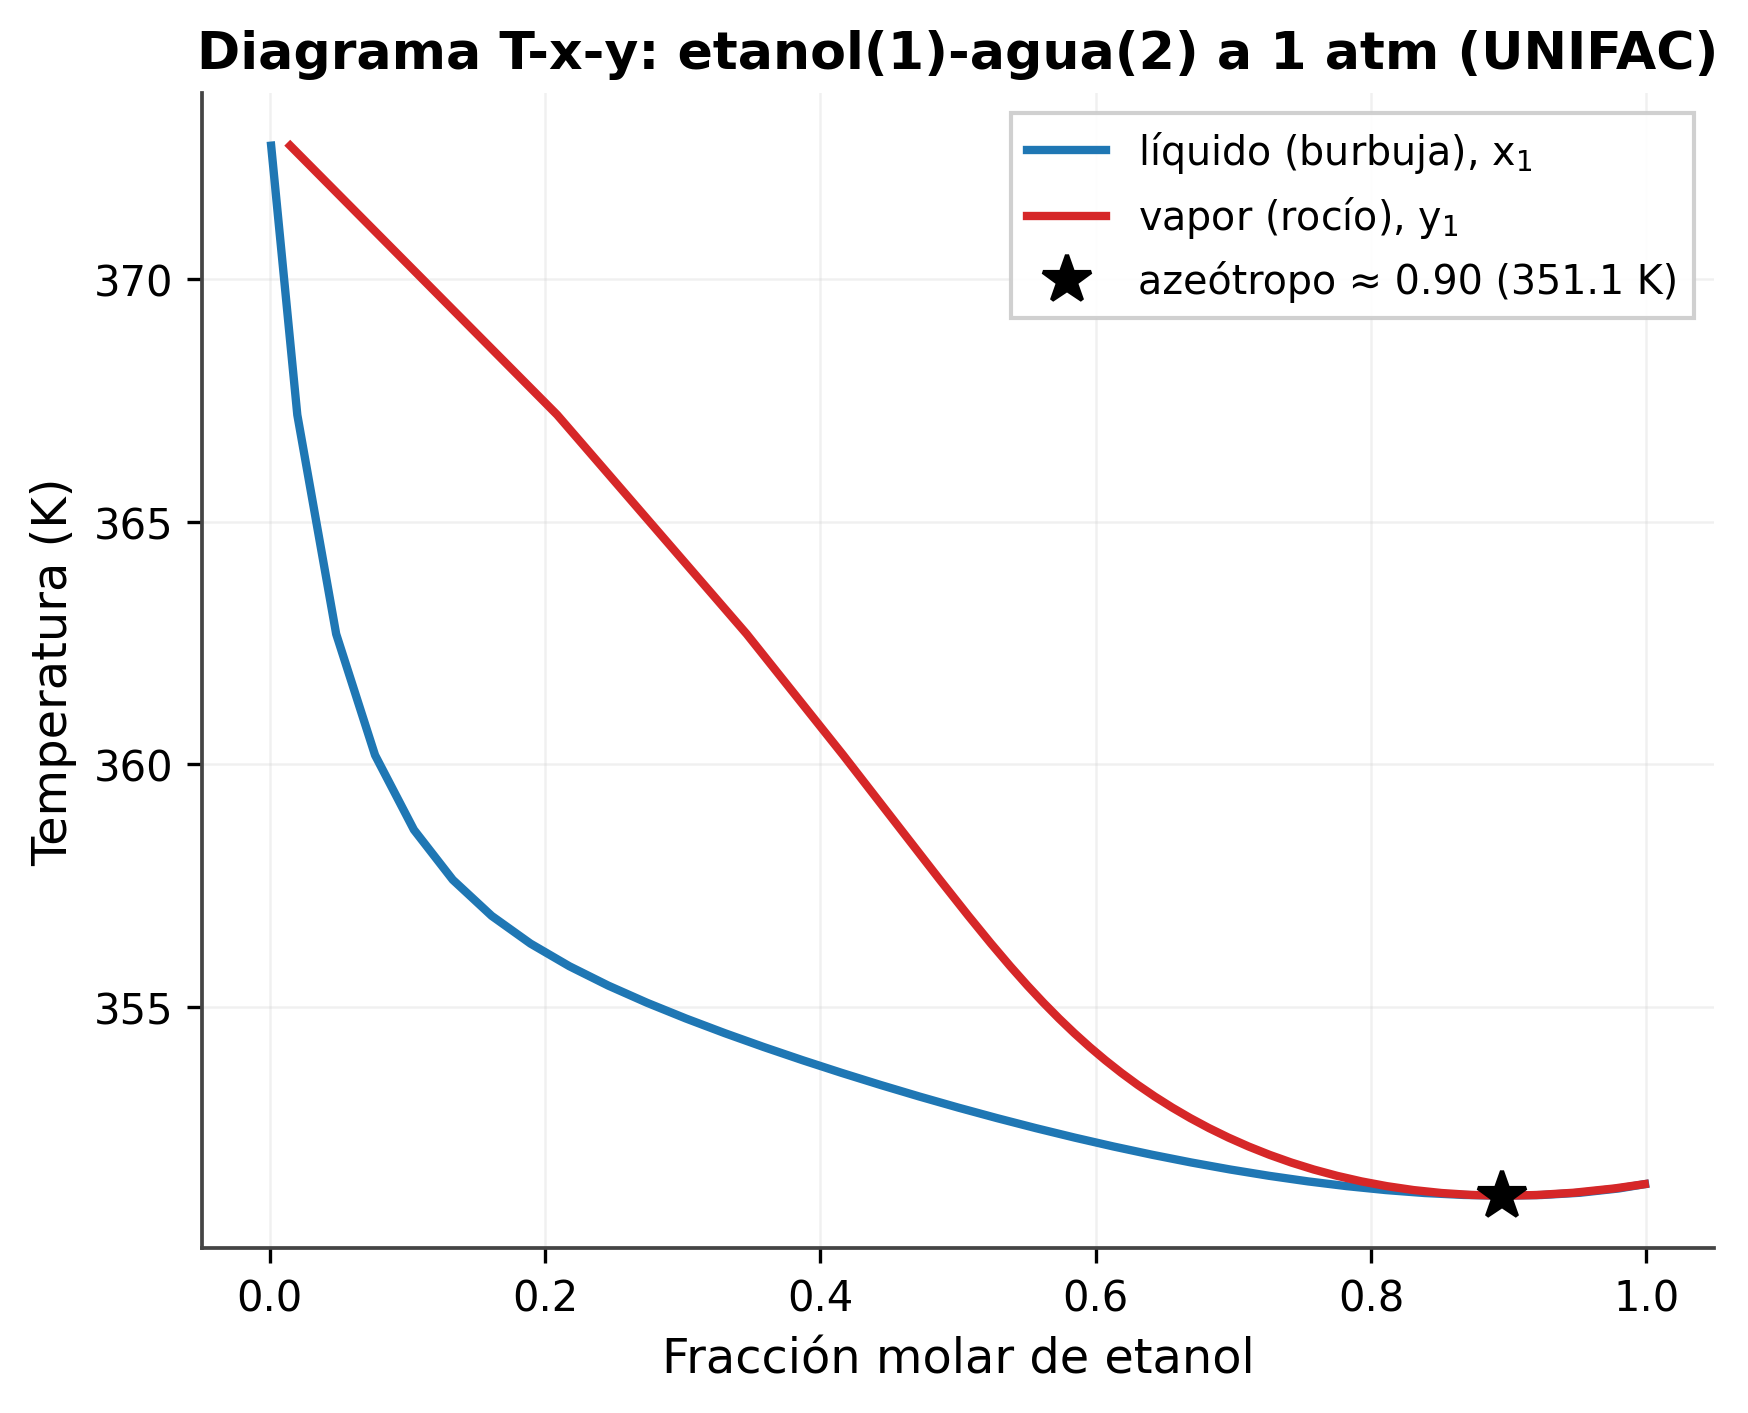
\includegraphics[width=0.72\textwidth]{figuras_exploratorias/A1_Txy_etanol_agua.png}
\caption{Diagrama T-x-y del sistema etanol-agua a 1~atm (UNIFAC). Las
curvas de burbuja y rocío se cruzan en un azeótropo de ebullición
mínima.}
\label{fig:A1}
\end{figure}

\begin{figure}[h]
\centering
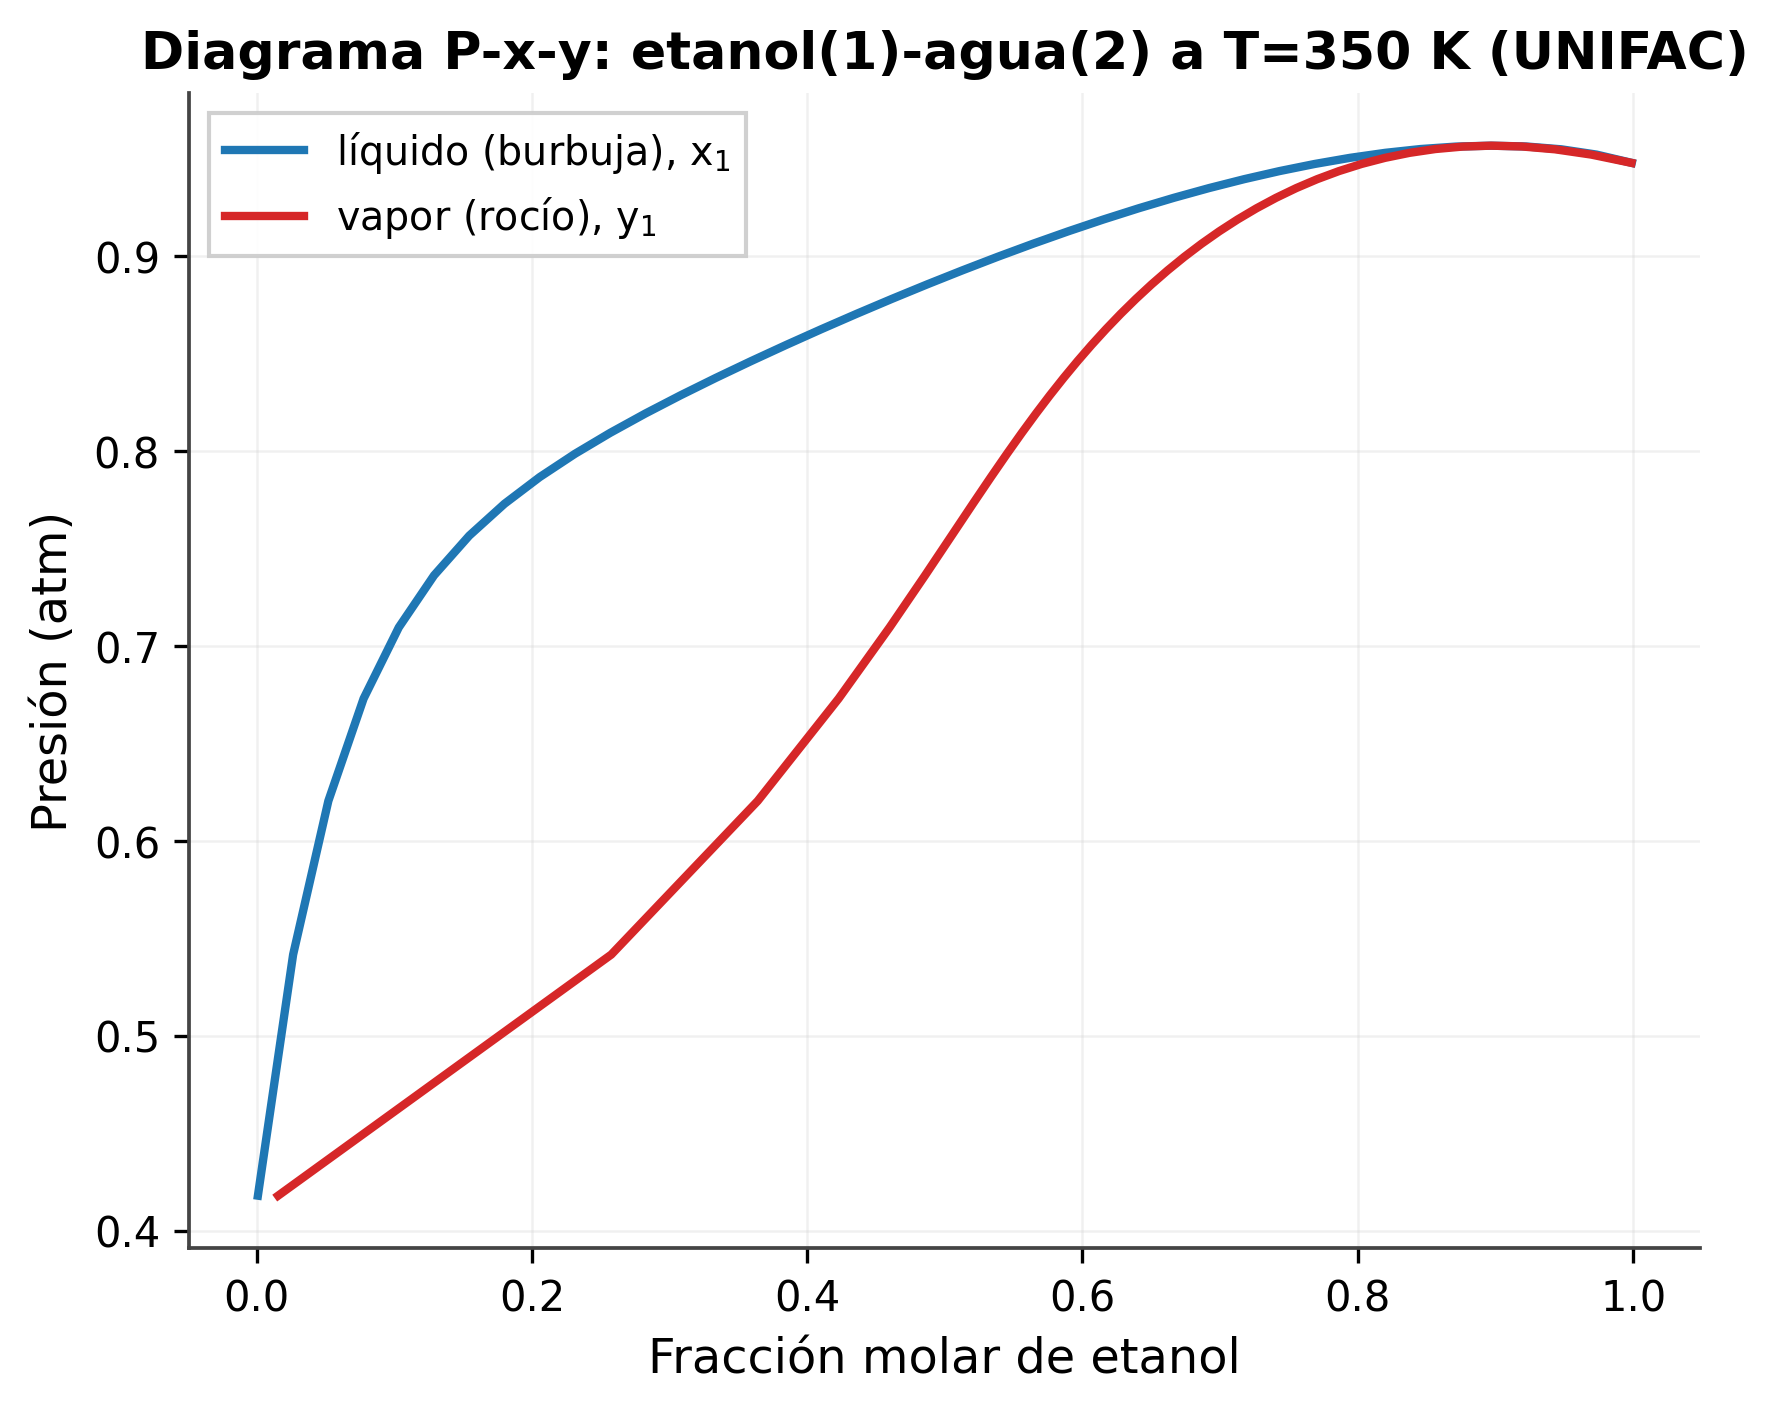
\includegraphics[width=0.72\textwidth]{figuras_exploratorias/A2_Pxy_etanol_agua.png}
\caption{Diagrama P-x-y a T=350~K. El azeótropo de T mínima en la
Fig.~\ref{fig:A1} corresponde, consistentemente, a un máximo de presión
aquí.}
\label{fig:A2}
\end{figure}

\begin{figure}[h]
\centering
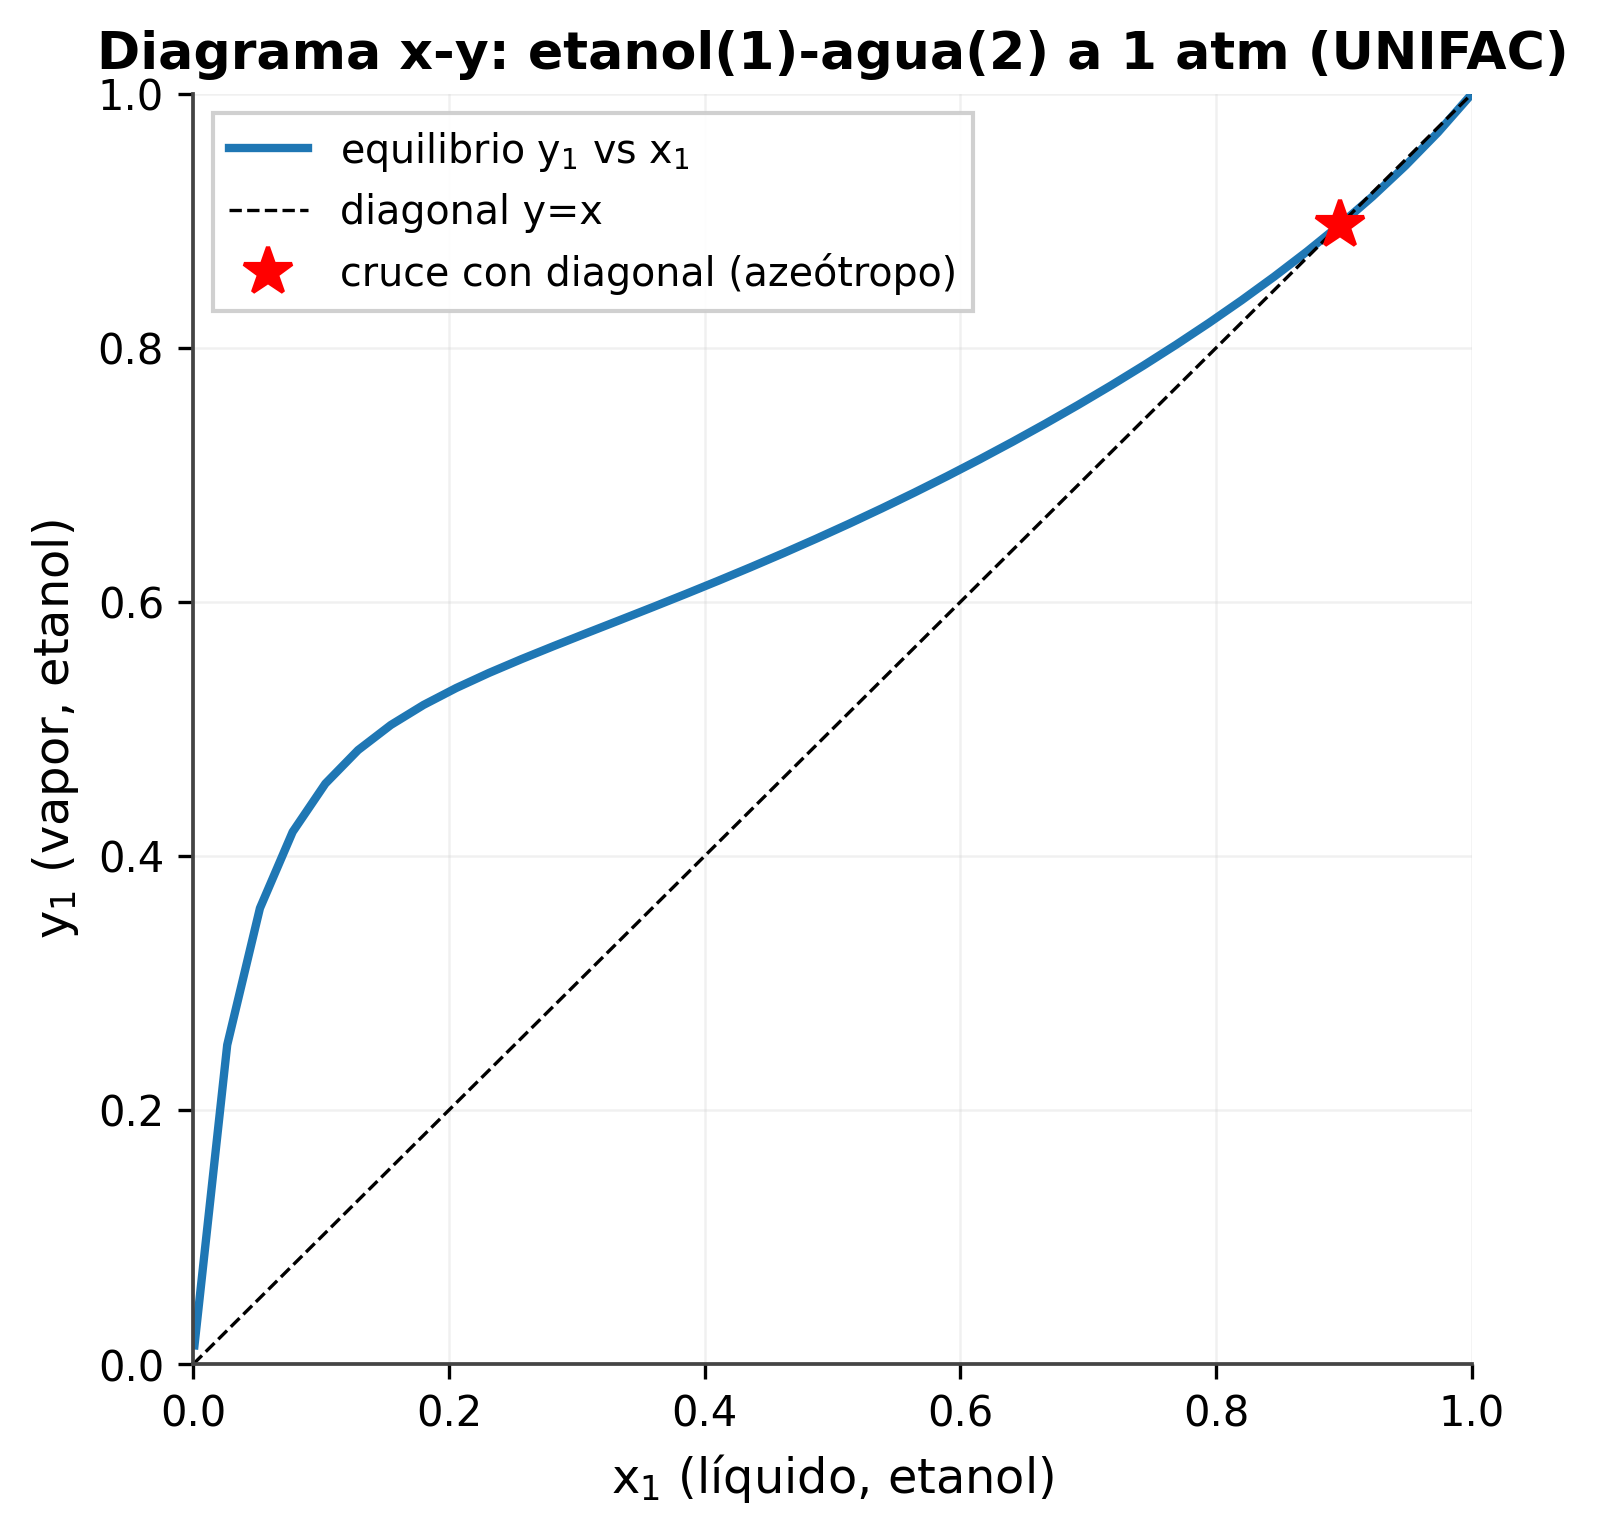
\includegraphics[width=0.58\textwidth]{figuras_exploratorias/A3_xy_etanol_agua.png}
\caption{Diagrama x-y a 1~atm. El cruce con la diagonal $y=x$ marca el
azeótropo.}
\label{fig:A3}
\end{figure}

\subsection{Validación: azeótropo etanol-agua}

El azeótropo etanol-agua a presión atmosférica es uno de los hechos
termodinámicos más citados en ingeniería química, ampliamente reportado
(p. ej. en colecciones de datos VLE como
\citet{gmehling1977}) en x$_{\text{et}} \approx 0.894$ (fracción molar)
y T $\approx 351.3$~K (78.15$^\circ$C). El modelo predice el azeótropo
en x$_{\text{et}}\approx 0.90$, T$\approx$351.1~K
(Fig.~\ref{fig:A1}--\ref{fig:A3}) -- una diferencia de apenas
$\sim$0.6\% en composición y 0.2~K en temperatura, notable considerando
que UNIFAC es un modelo \emph{predictivo} (sin ningún parámetro
ajustado a este sistema específico). Esta es la validación cuantitativa
más fuerte de este documento.

% =====================================================================
\section{Equilibrio líquido-líquido: domo de solución regular}
\label{sec:lle}
% =====================================================================

Para ilustrar el equilibrio líquido-líquido (LLE), se usó un sistema
binario ficticio con un modelo de solución regular cuyo parámetro de
interacción depende de la temperatura de la forma termodinámicamente
estándar $\Lambda(T)=\Omega/(RT)$, con $\Omega=6000$~J/mol elegido
\textbf{ilustrativamente} (no corresponde a ningún par de compuestos
reales). Para una solución regular simétrica, esta forma funcional
produce una temperatura crítica superior de solución (UCST) exacta:
$T_c = \Omega/(2R) \approx 360.8$~K, confirmada analíticamente por el
cálculo (Fig.~\ref{fig:B1}).

\begin{figure}[h]
\centering
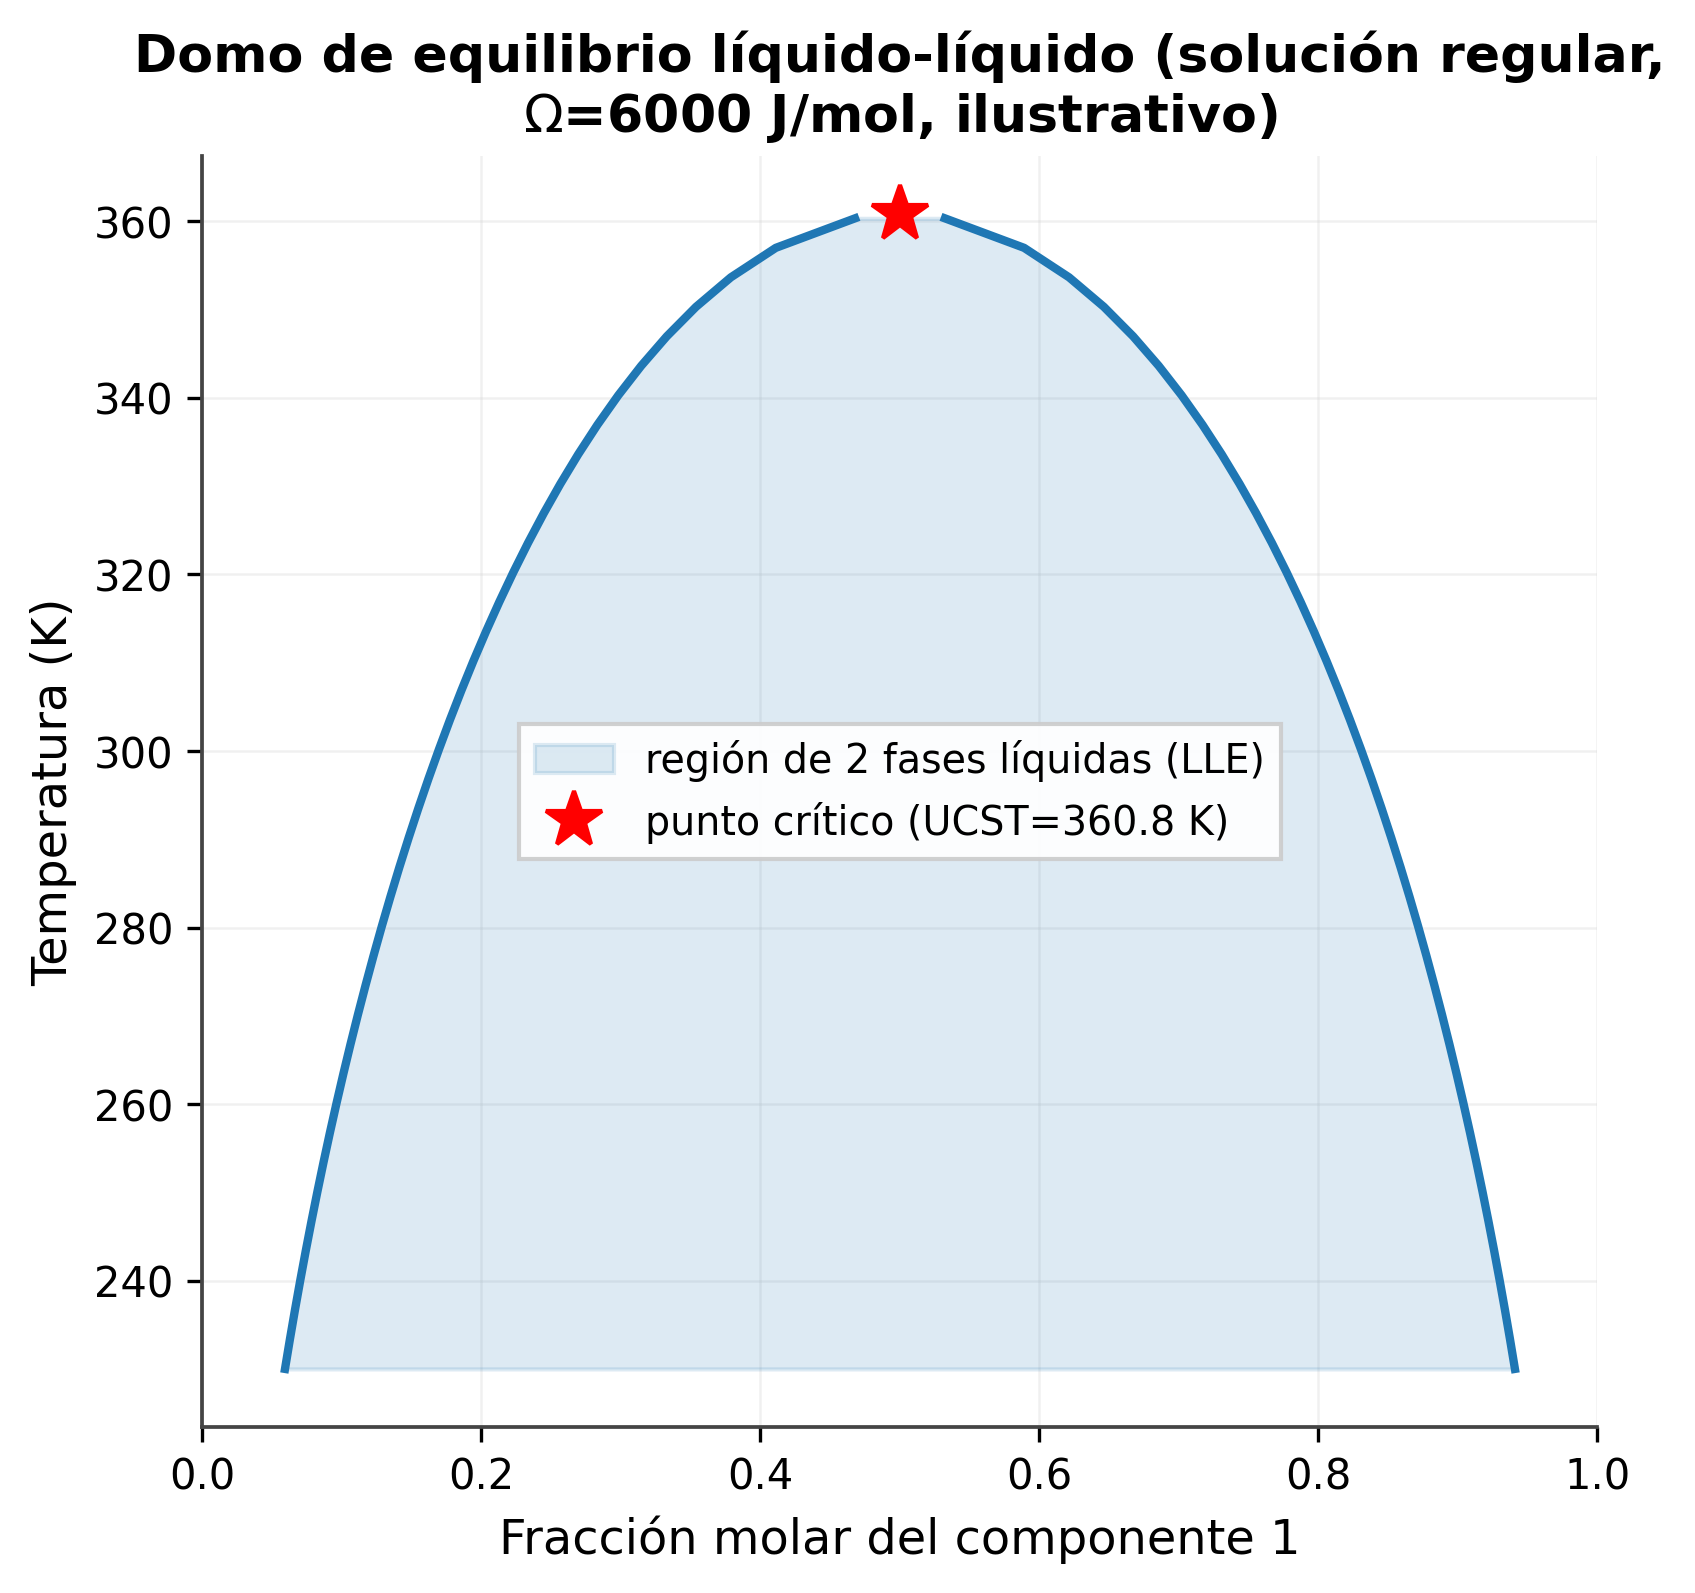
\includegraphics[width=0.62\textwidth]{figuras_exploratorias/B1_LLE_binodal.png}
\caption{Domo de equilibrio líquido-líquido: composiciones de las dos
fases en equilibrio (binodal) en función de T. El domo es exactamente
simétrico respecto a x=0.5, como corresponde a una solución regular
simétrica.}
\label{fig:B1}
\end{figure}

Esta figura es una \textbf{demostración matemática correcta} del
modelo de solución regular y de los solvers de equilibrio de fases,
\emph{no} una predicción validada contra un sistema químico real.

% =====================================================================
\section{Síntesis de MTBE: equilibrio químico y de fases simultáneo}
\label{sec:mtbe}
% =====================================================================

Sistema reactivo isobuteno + metanol $\rightleftharpoons$ MTBE (ver
\texttt{ejemplo\_mtbe.py}, datos termodinámicos ilustrativos
documentados allí). Se exploran cuatro aspectos: el diagrama T-x-y con
reacción, el isobuteno remanente por fase, la trayectoria de
composición en un diagrama ternario, y la fracción de fase vapor en
función de la presión.

\begin{figure}[h]
\centering
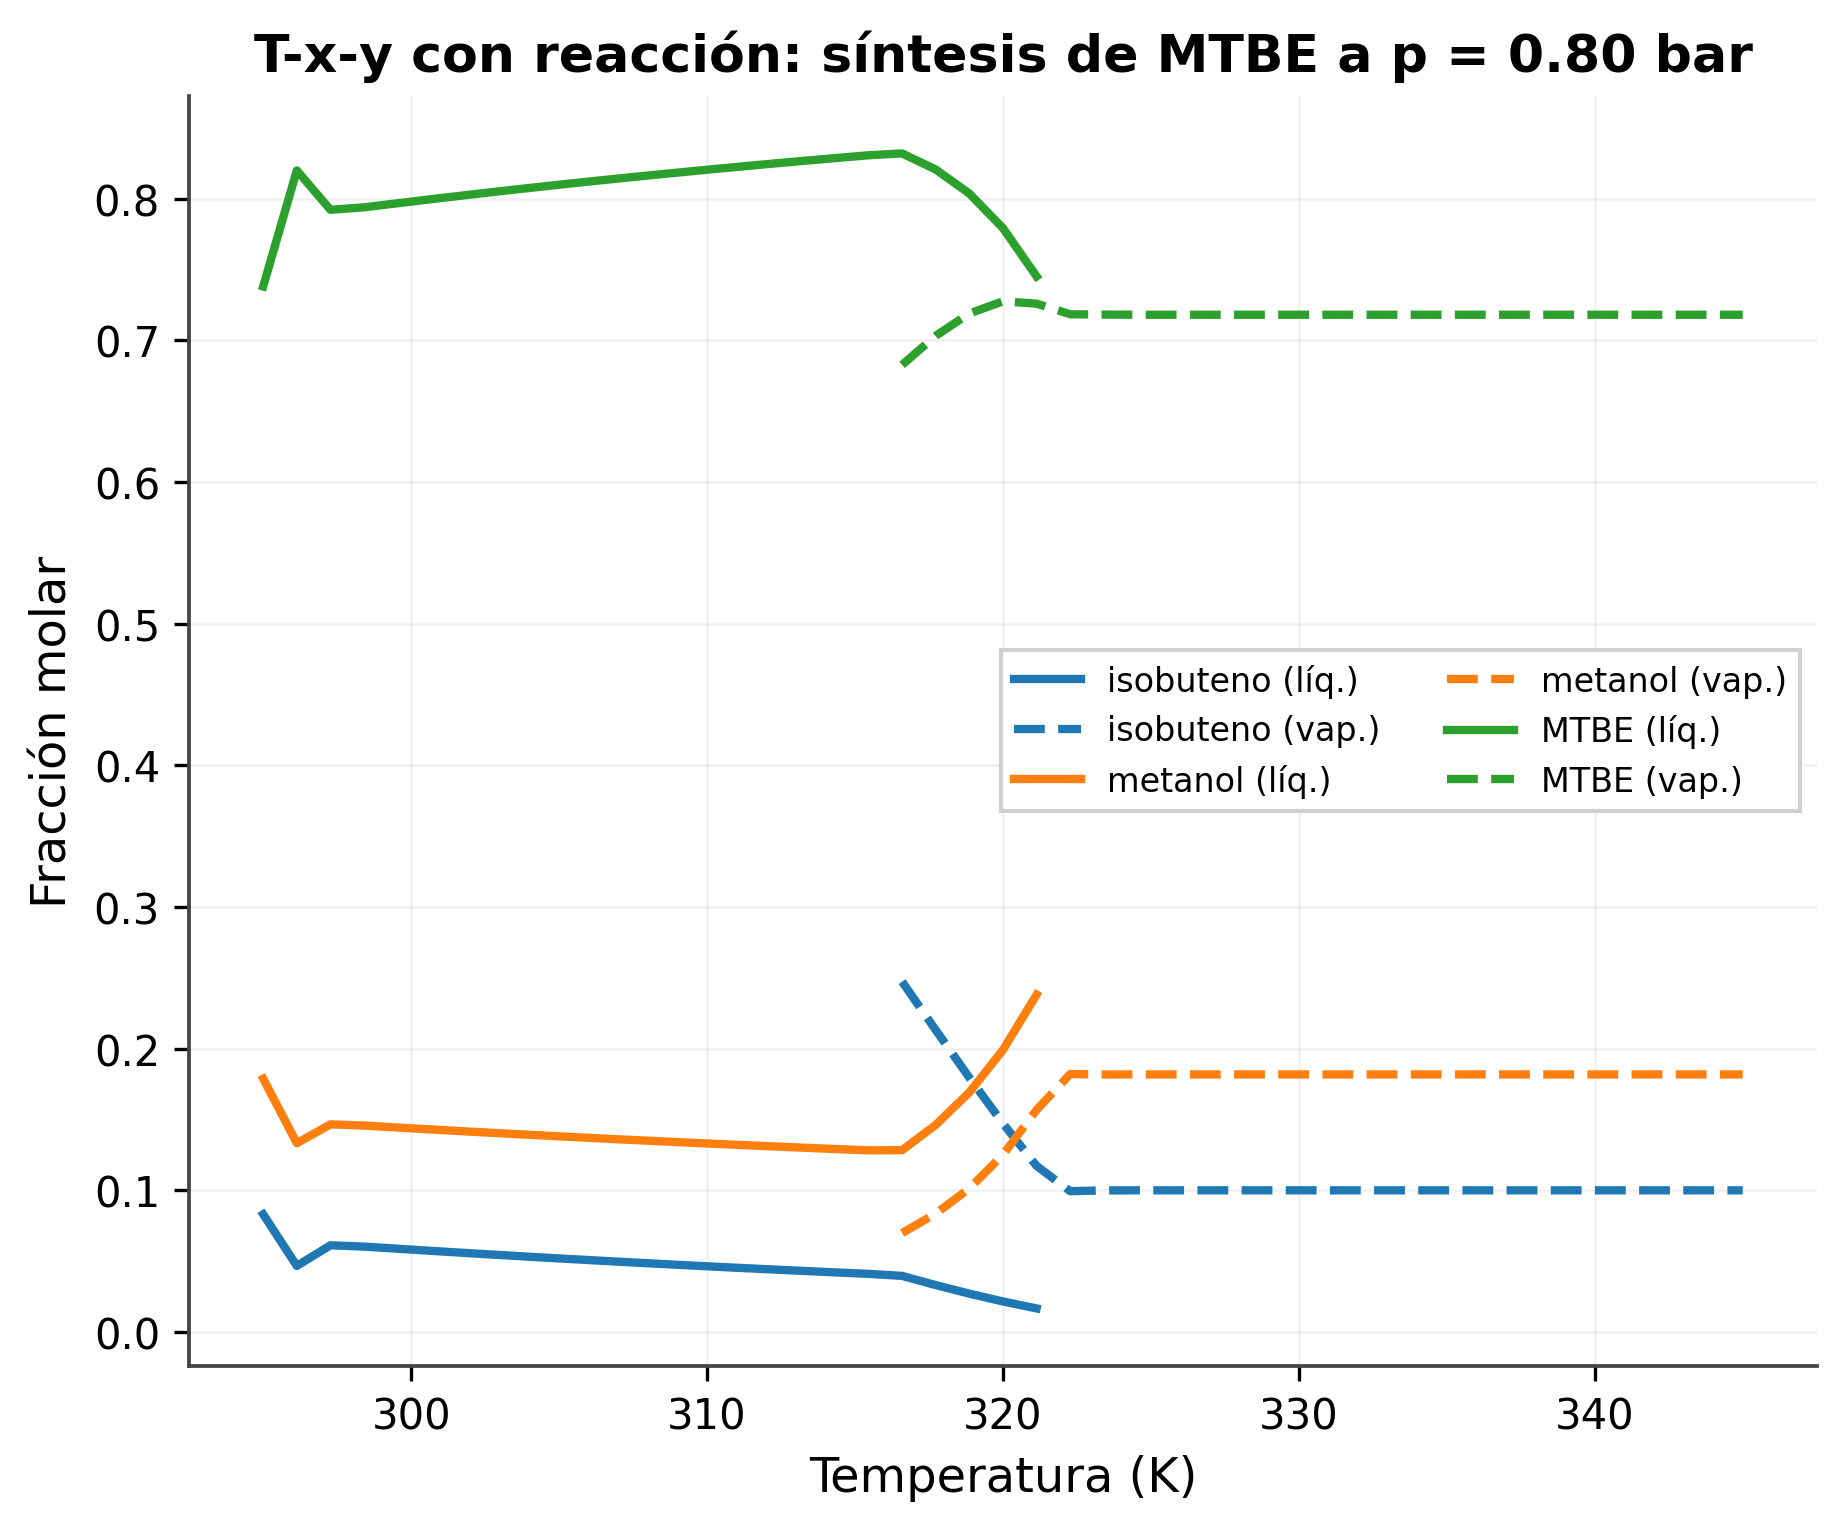
\includegraphics[width=0.75\textwidth]{figuras_exploratorias/C1_Txy_mtbe.png}
\caption{T-x-y con reacción química a p=0.80~bar. La ventana de
coexistencia líquido-vapor es notablemente angosta ($\sim$317--322~K):
fuera de ella, una de las dos fases colapsa a cantidad despreciable.}
\label{fig:C1}
\end{figure}

\begin{figure}[h]
\centering
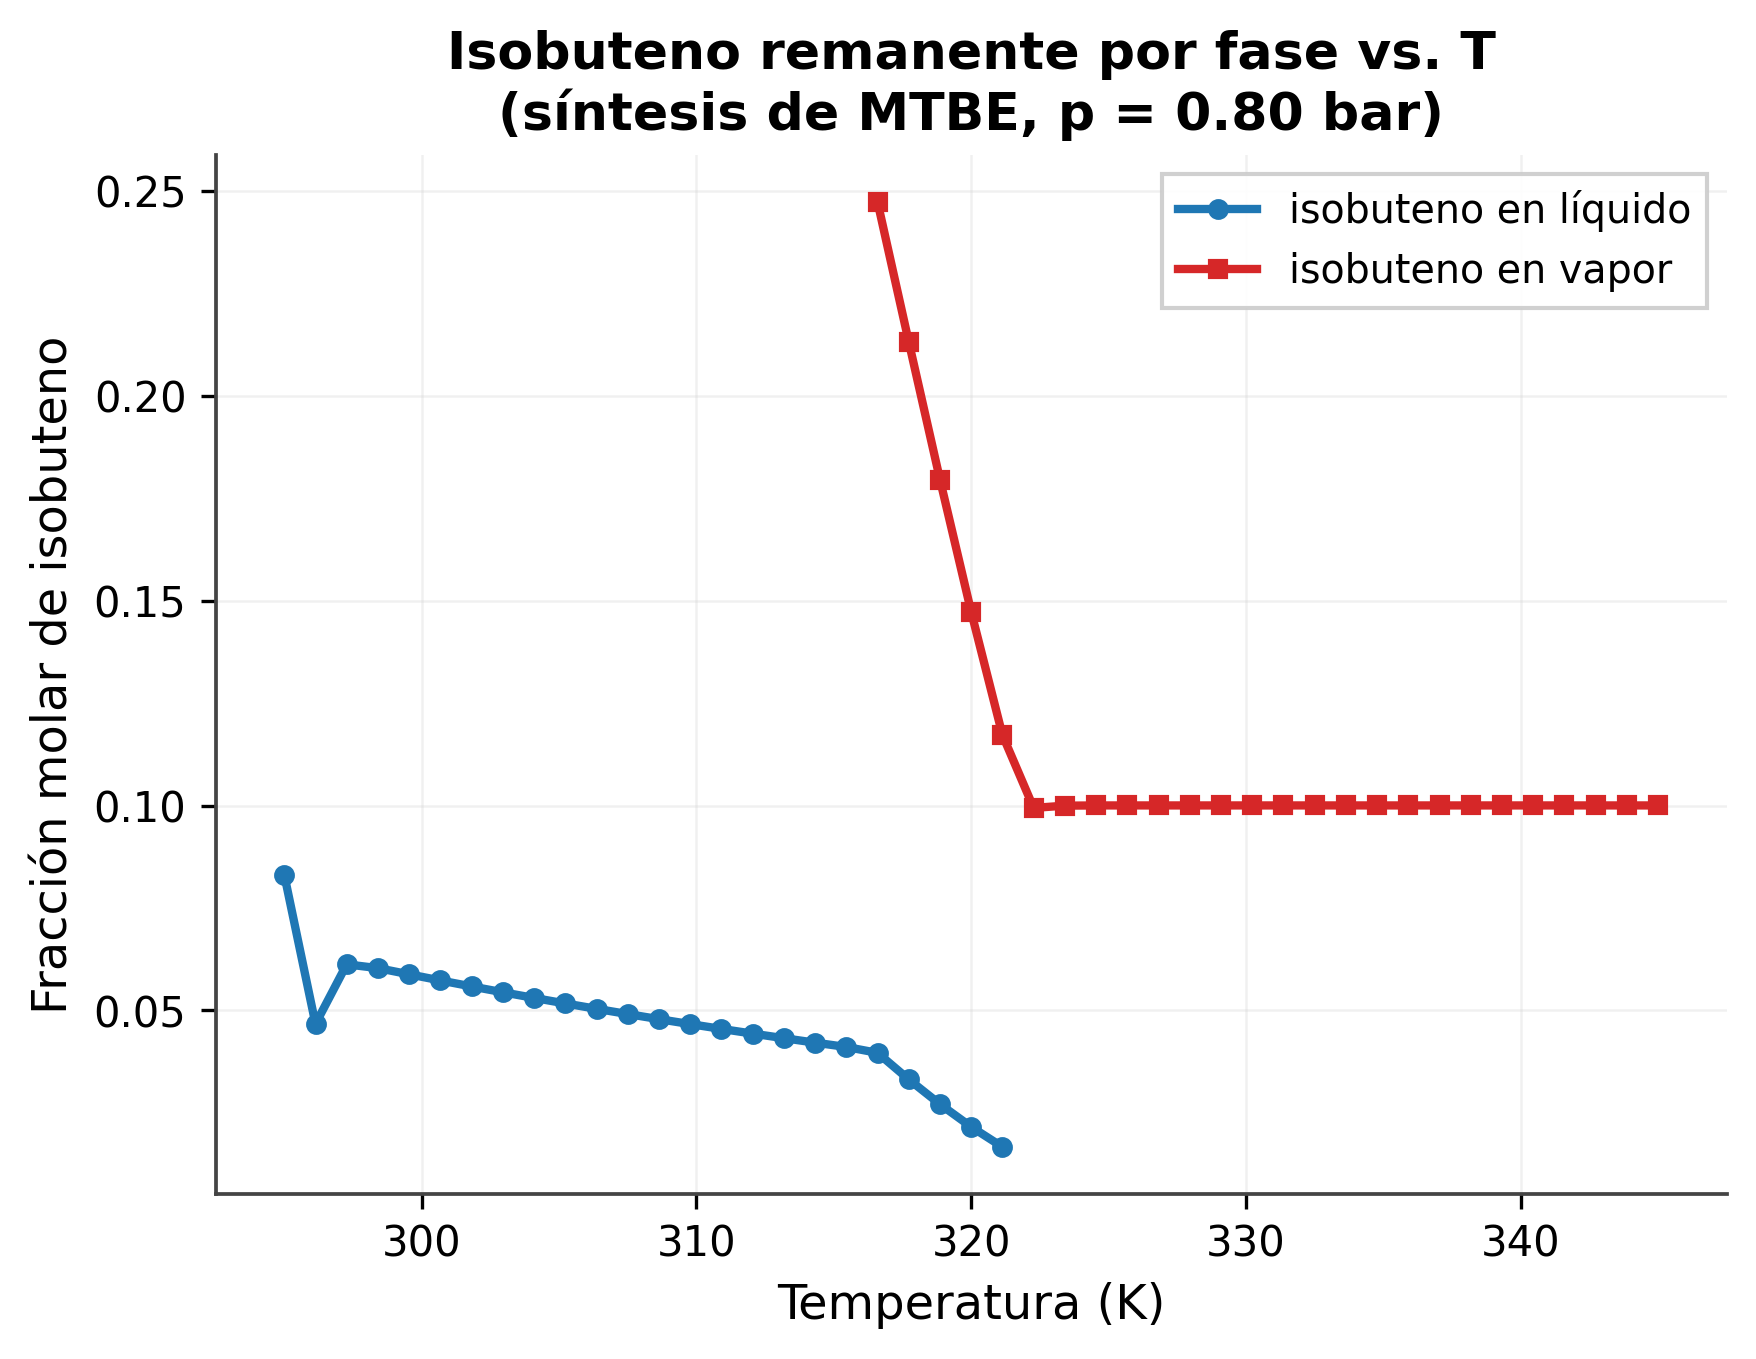
\includegraphics[width=0.68\textwidth]{figuras_exploratorias/C2_isobuteno_vs_T_mtbe.png}
\caption{Isobuteno remanente en cada fase vs. T. El salto entre las
curvas marca la ventana de transición de la Fig.~\ref{fig:C1}.}
\label{fig:C2}
\end{figure}

\begin{figure}[h]
\centering
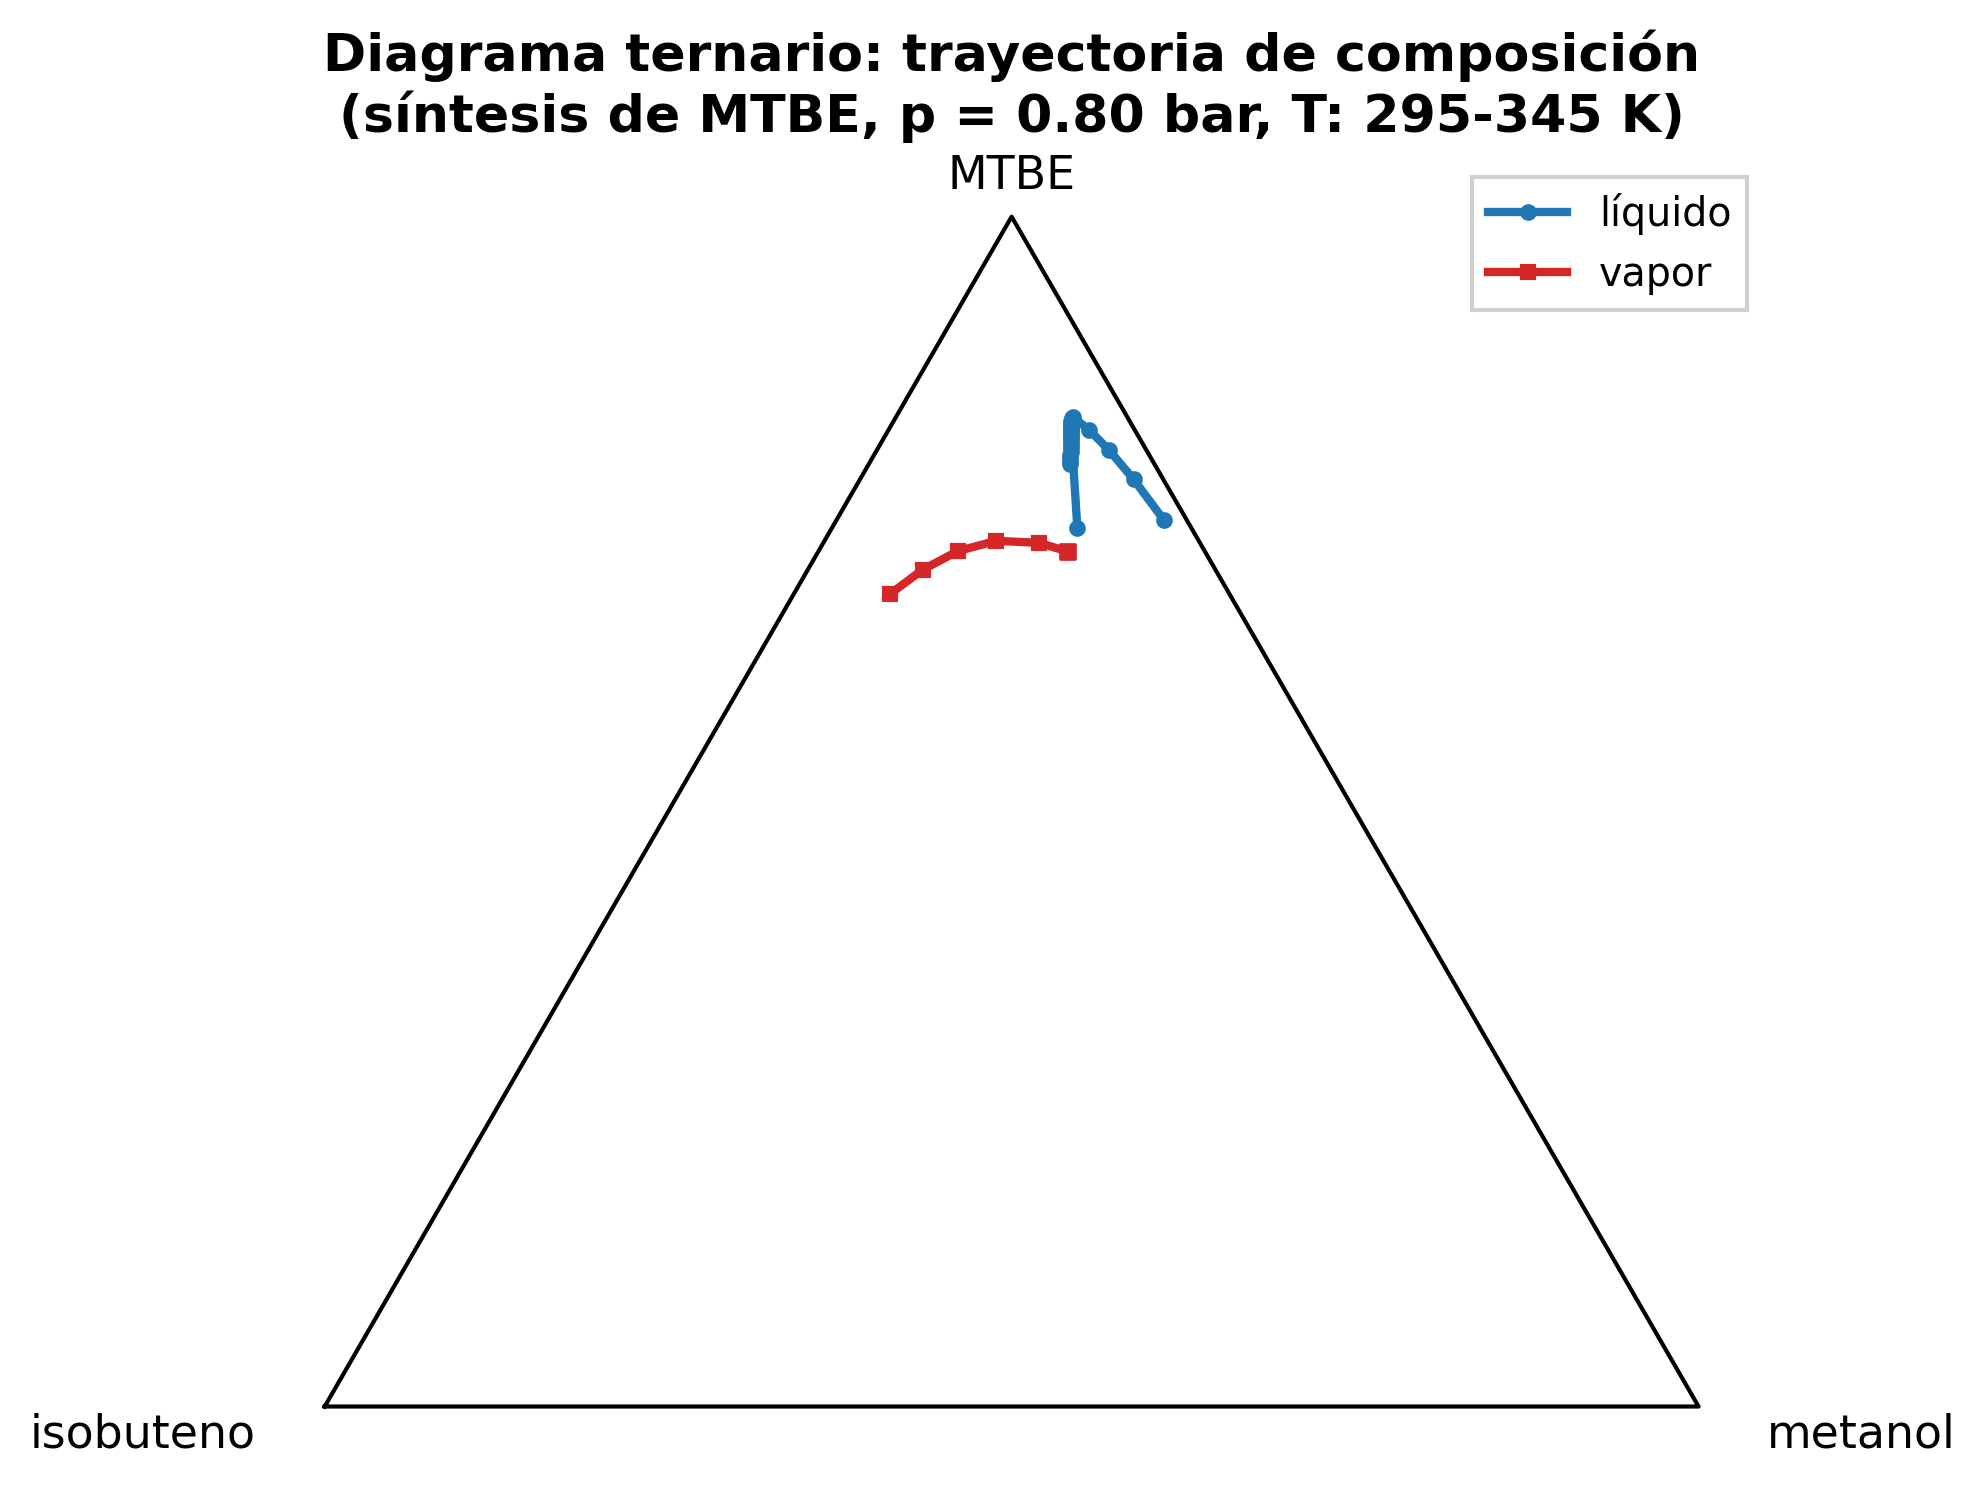
\includegraphics[width=0.55\textwidth]{figuras_exploratorias/C3_ternario_mtbe.png}
\caption{Diagrama ternario isobuteno-metanol-MTBE: trayectoria de
composición líquida y vapor conforme T recorre 295--345~K.}
\label{fig:C3}
\end{figure}

\begin{figure}[h]
\centering
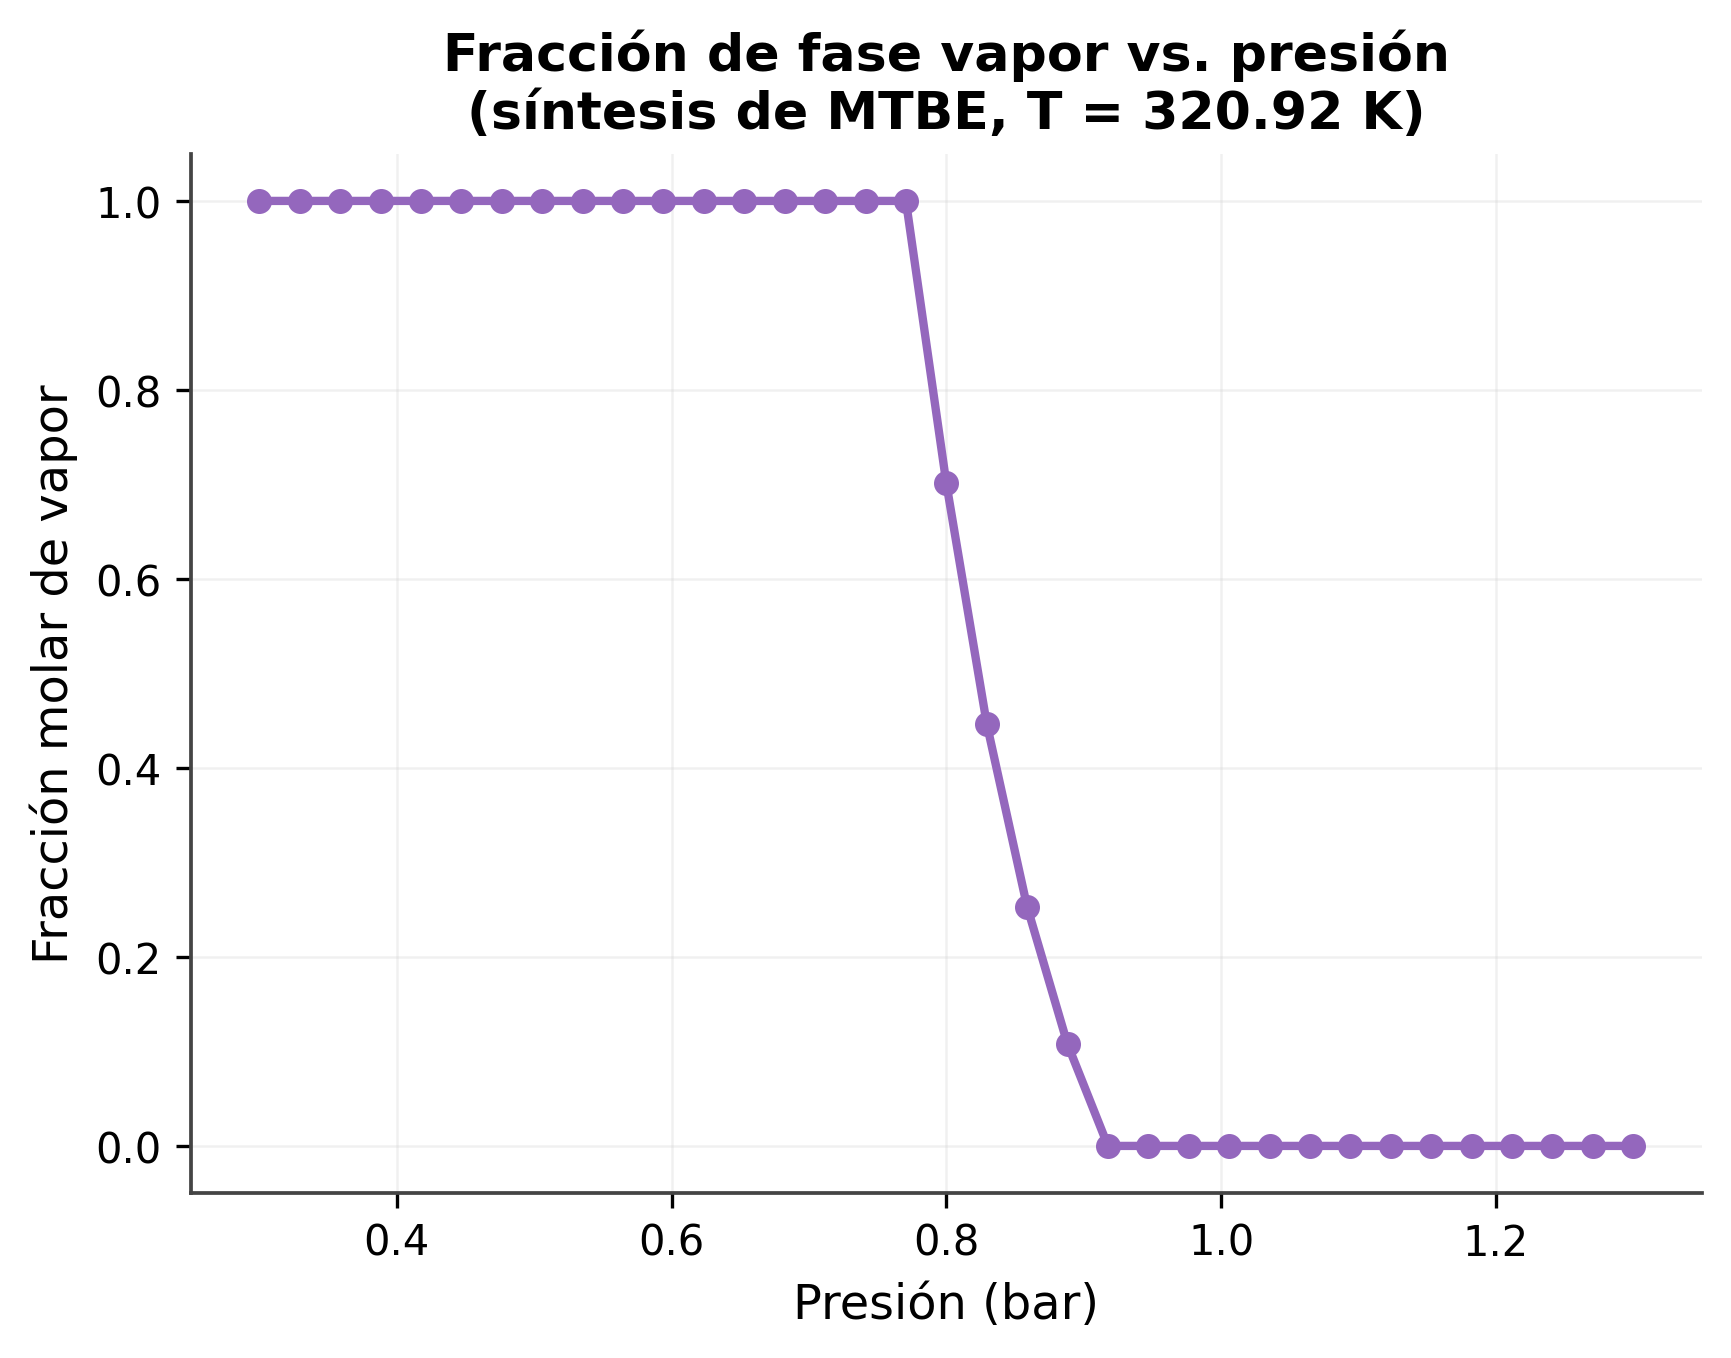
\includegraphics[width=0.68\textwidth]{figuras_exploratorias/C4_fraccion_vapor_vs_P_mtbe.png}
\caption{Fracción de fase vapor vs. presión a T=320.92~K: una curva de
flash suave y monotónica, de 100\% vapor a baja presión hasta 100\%
líquido por encima de $\sim$0.9~bar.}
\label{fig:C4}
\end{figure}

\subsection{Observación: ventana de transición angosta}

Un hallazgo notable del modelo (Fig.~\ref{fig:C1}--\ref{fig:C2}) es que
la ventana de temperatura donde coexisten ambas fases a presión fija es
mucho más angosta ($\sim$5~K) que la ventana de presión a temperatura
fija (Fig.~\ref{fig:C4}, $\sim$0.6~bar). Esto es consistente con que
$K_{\text{eq}}$ se mantiene constante en este modelo (no depende de T,
ver advertencia en \texttt{ejemplo\_mtbe.py}): la composición de
equilibrio químico no se ajusta con T, por lo que el equilibrio de
fases se vuelve el único grado de libertad que responde a T, haciendo
la transición más abrupta que si $K_{\text{eq}}(T)$ también variara
suavemente (como en el caso de esterificación, Sección~\ref{sec:esterificacion}).

% =====================================================================
\section{Esterificación ácido acético/etanol: equilibrio reactivo}
\label{sec:esterificacion}
% =====================================================================

A diferencia del sistema MTBE, aquí $K_{\text{eq}}(T)$ sí varía
suavemente con T (van't Hoff, ya validado en \texttt{documentacion.pdf}
contra \citet{smithvannessabbott}), lo que produce una transición de
fase considerablemente más suave.

\begin{figure}[h]
\centering
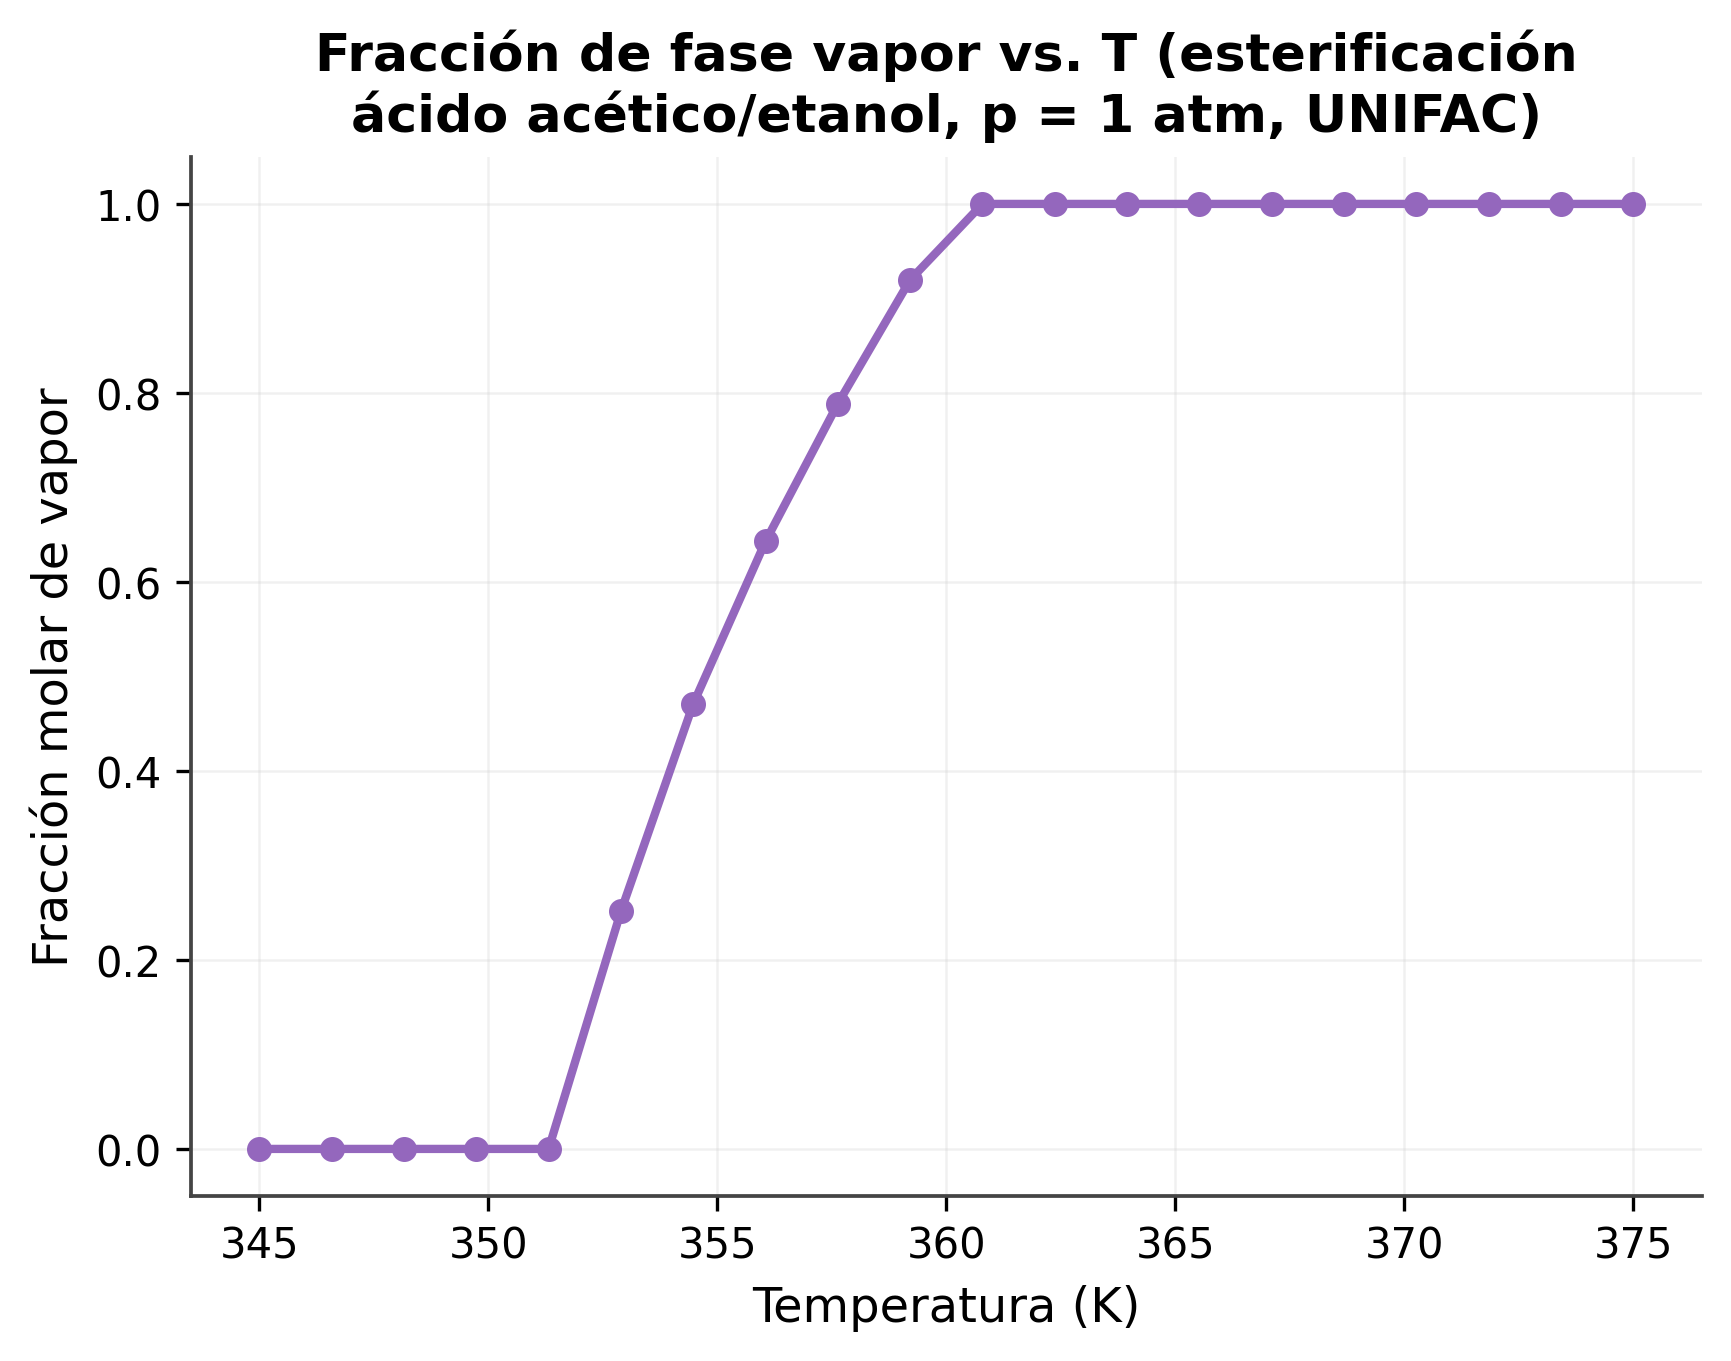
\includegraphics[width=0.68\textwidth]{figuras_exploratorias/D1_fraccion_vapor_vs_T_esterificacion.png}
\caption{Fracción de fase vapor vs. T a 1~atm (UNIFAC). La transición
ocurre en una ventana de $\sim$10~K (351--361~K), notablemente más
ancha que la del sistema MTBE (Fig.~\ref{fig:C1}), consistente con la
discusión de la Sección~\ref{sec:mtbe}.}
\label{fig:D1}
\end{figure}

\begin{figure}[h]
\centering
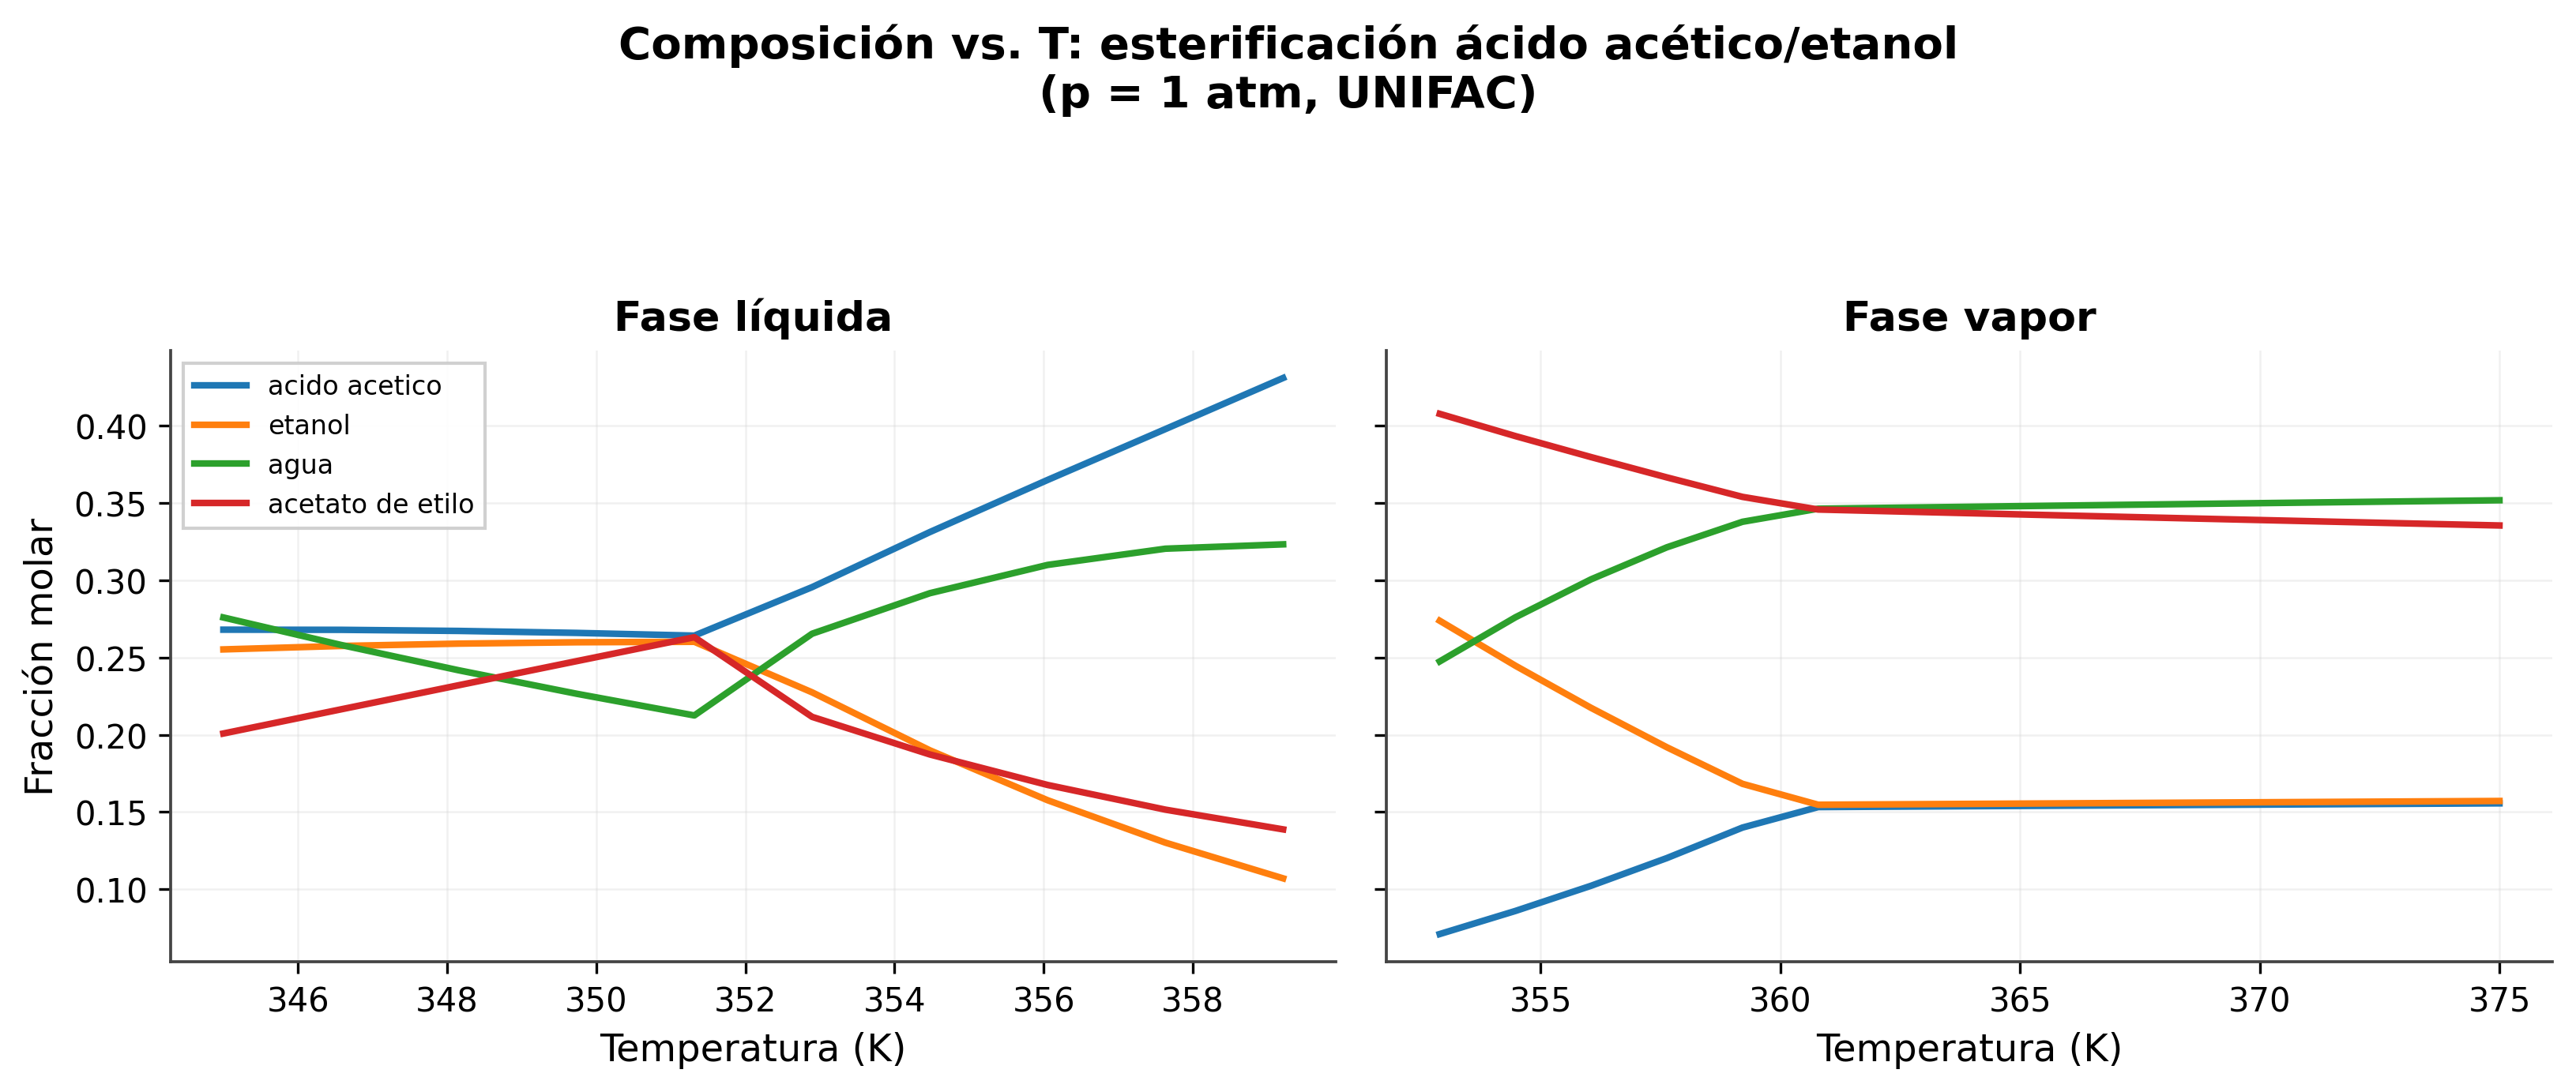
\includegraphics[width=0.95\textwidth]{figuras_exploratorias/D2_especies_vs_T_esterificacion.png}
\caption{Composición de cada fase vs. T. El ácido acético se concentra
progresivamente en el líquido al aumentar T (menos volátil, en este
modelo), mientras que agua y acetato de etilo dominan el vapor.}
\label{fig:D2}
\end{figure}

% =====================================================================
\section{Combustión y oxidación: potenciales de elemento}
\label{sec:combustion}
% =====================================================================

Estos perfiles usan el mismo formalismo de potenciales de elemento
(minimización de Gibbs no estequiométrica, Ec.~3.6 y 3.14 de
\citet{tsanas2018}) que el resto del proyecto, aplicado a una sola fase
gas ideal con múltiples especies -- el mismo enfoque usado por
\citet{binous2022} para sus casos de combustión de hidracina y
propano. Los datos termoquímicos (ver \texttt{combustion\_gibbs.py})
son valores aproximados de entalpía y energía de Gibbs de formación
estándar (298~K), típicos de tablas NIST-JANAF, usados con la
aproximación de capacidad calorífica de reacción nula ($\Delta C_p
\approx 0$): esto captura la tendencia cualitativa correcta pero no
debe usarse para diseño.

\subsection{Disociación de CO$_2$ y H$_2$O}

\begin{figure}[h]
\centering
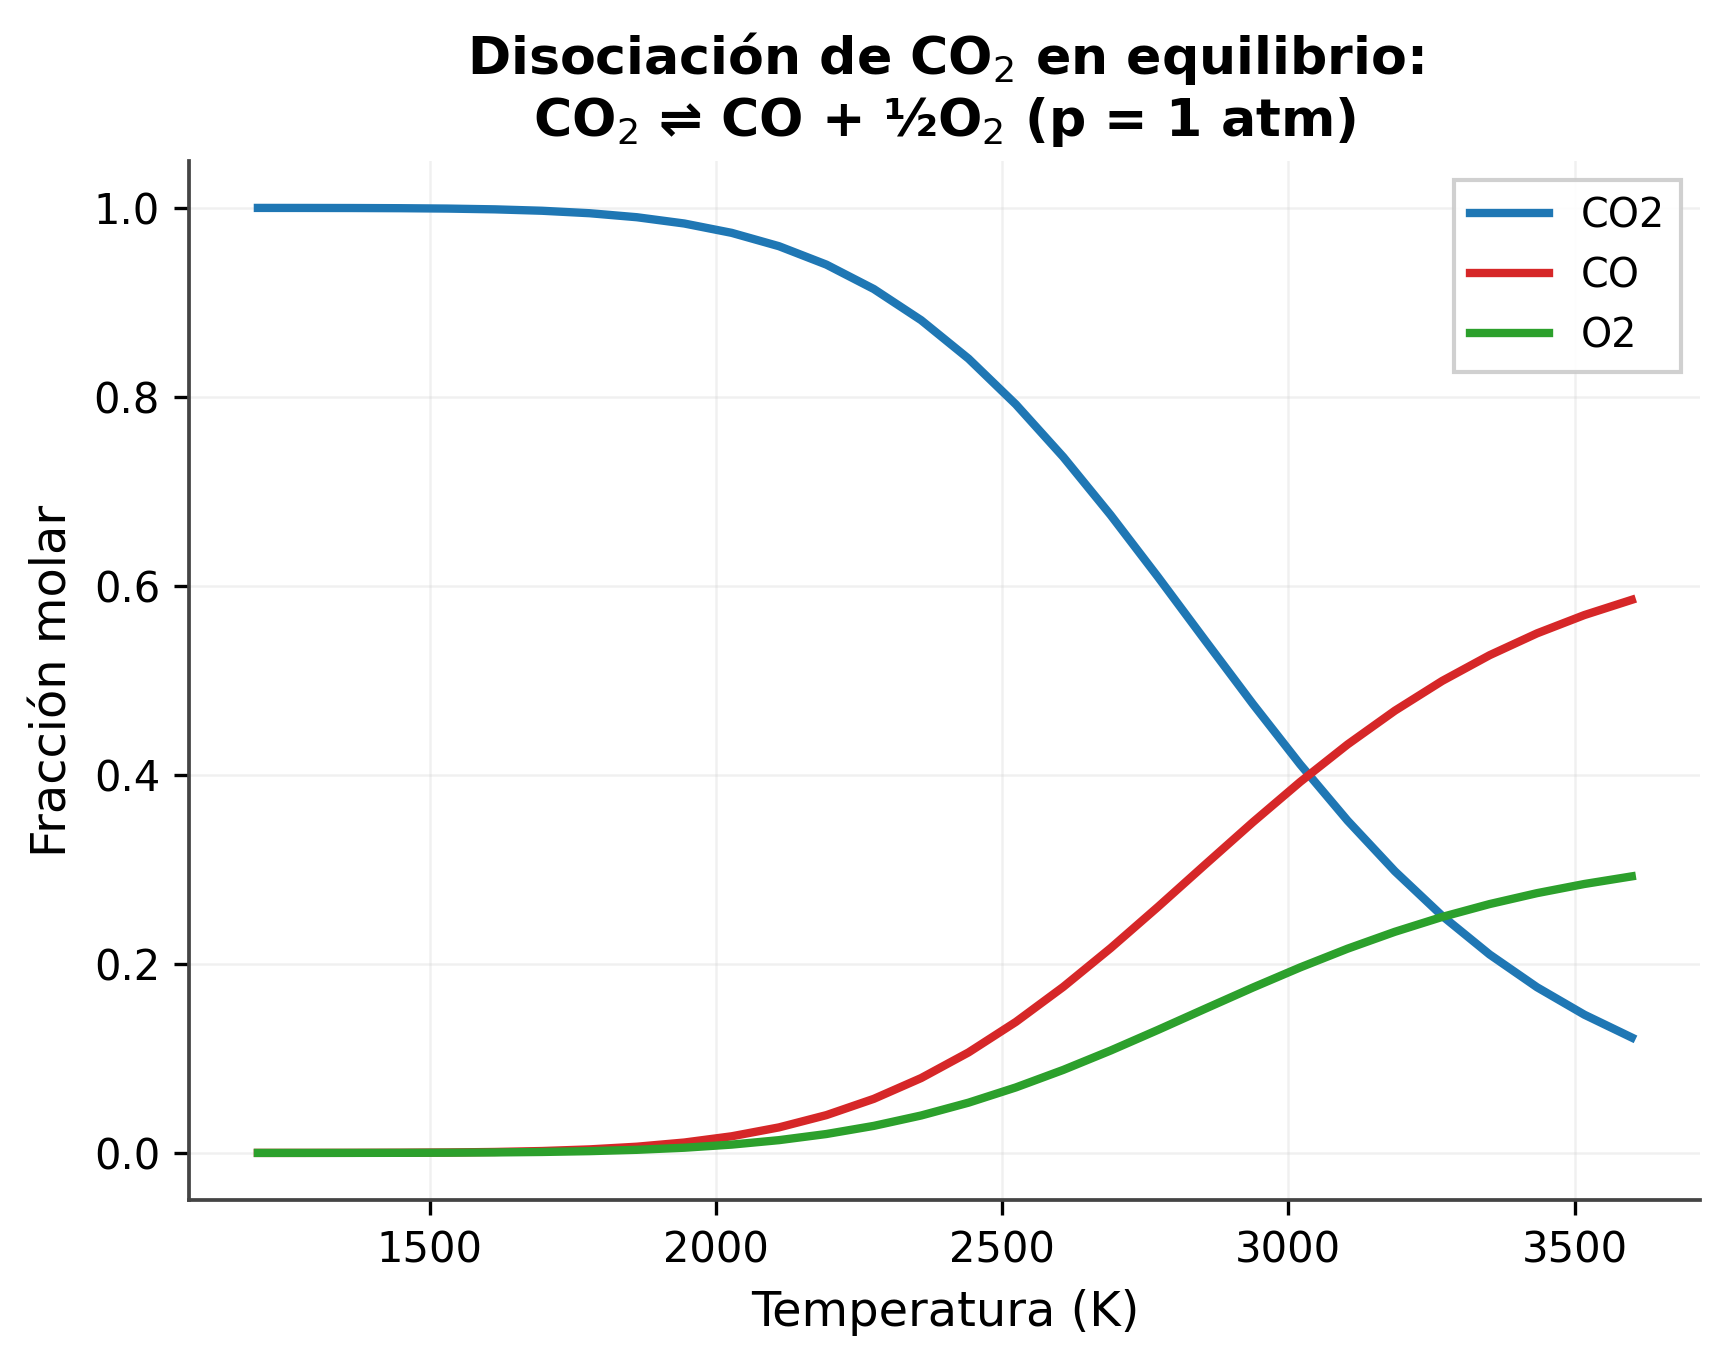
\includegraphics[width=0.68\textwidth]{figuras_exploratorias/E1_disociacion_CO2.png}
\caption{Disociación de CO$_2$ (CO$_2\rightleftharpoons$CO+$\frac12$O$_2$)
en función de T a 1~atm: disociación despreciable por debajo de
$\sim$1800~K, con un cambio de régimen pronunciado y
Le~Chatelier-consistente hacia 3000--3500~K.}
\label{fig:E1}
\end{figure}

\begin{figure}[h]
\centering
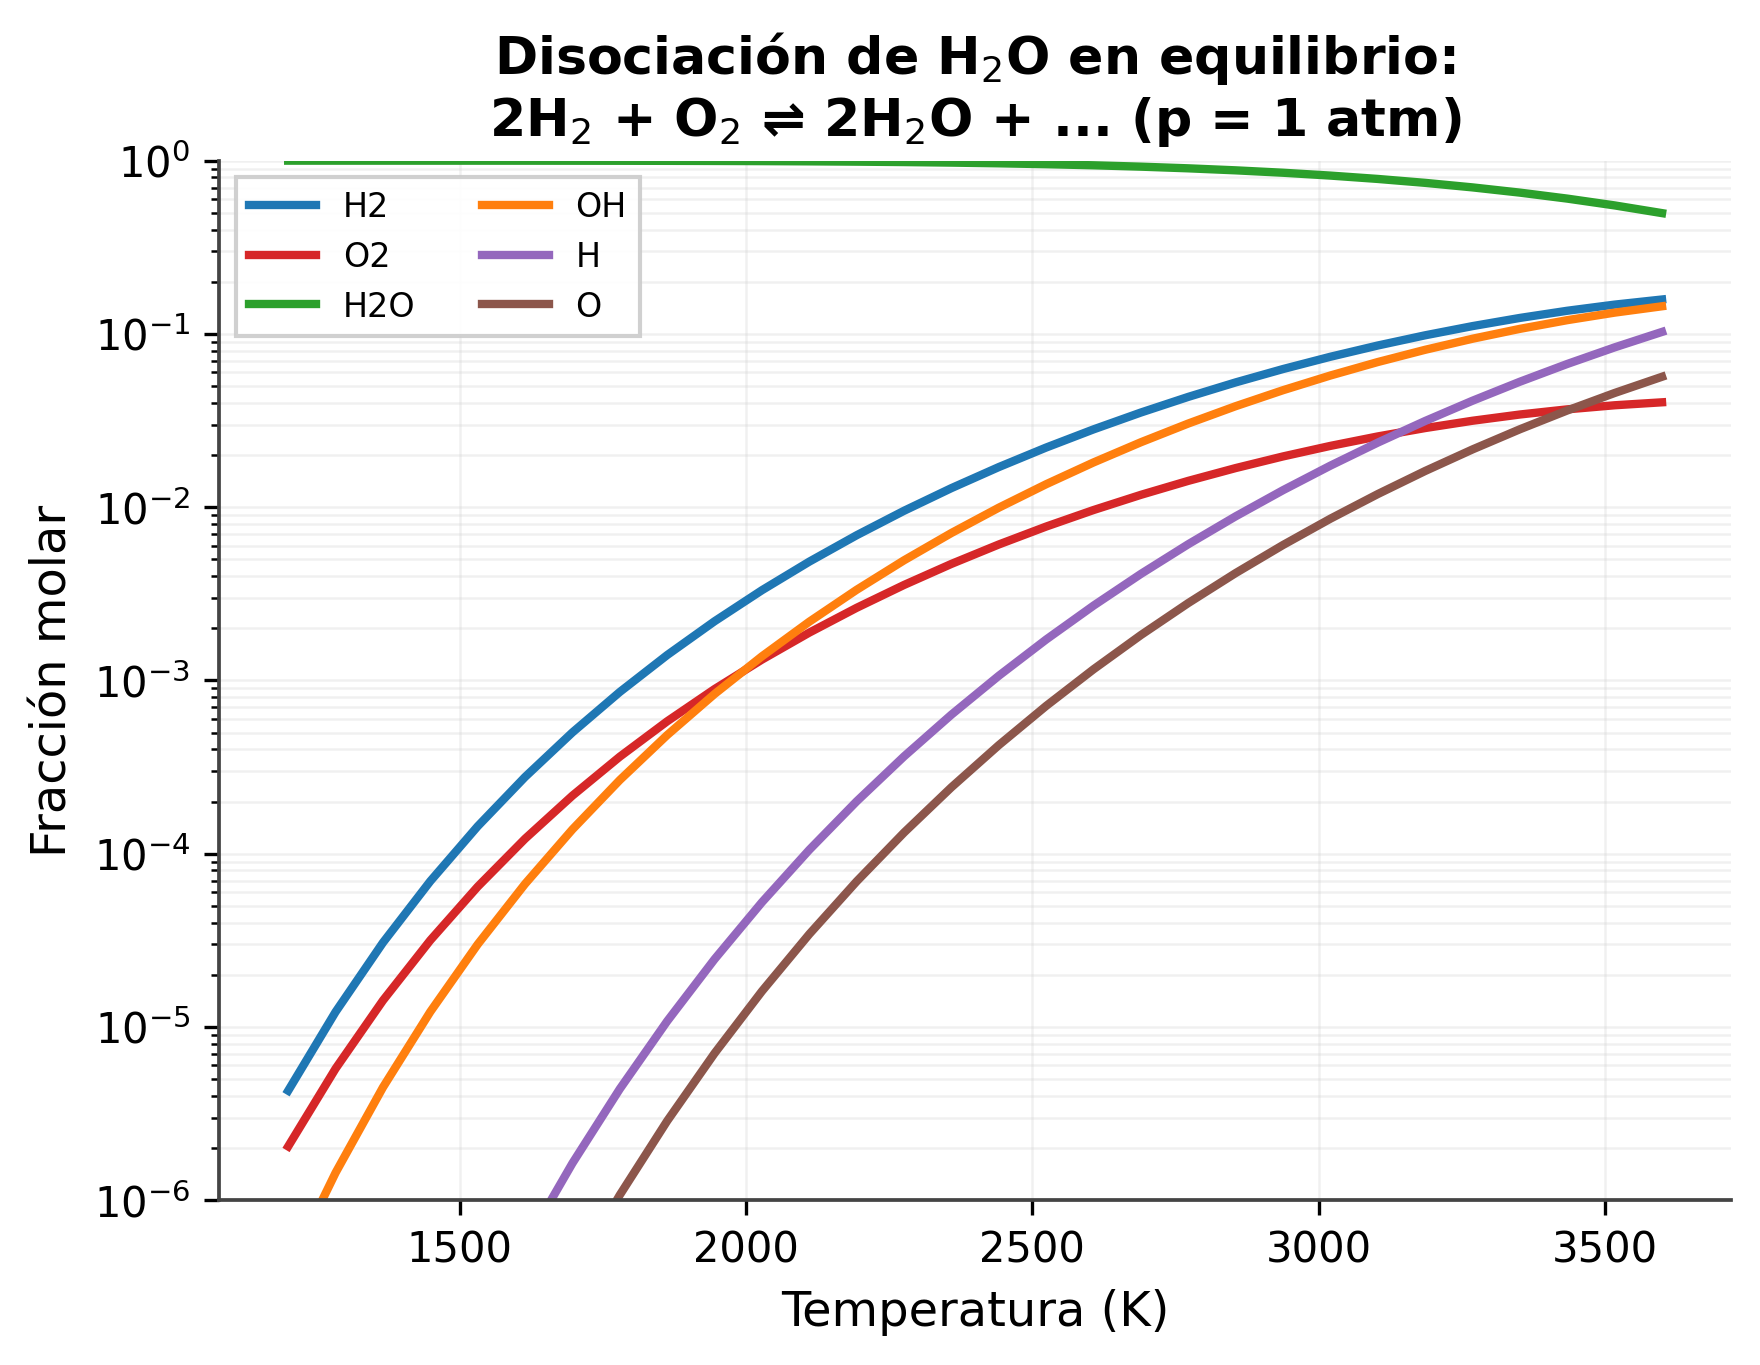
\includegraphics[width=0.68\textwidth]{figuras_exploratorias/E2_disociacion_H2O.png}
\caption{Disociación de H$_2$O en sus productos de alta temperatura
(H$_2$, O$_2$, OH, H, O), escala logarítmica. El orden de aparición de
las especies traza (H$_2$/O$_2$ primero, luego OH, luego H/O) es
consistente con las energías de disociación relativas.}
\label{fig:E2}
\end{figure}

\subsection{Productos de combustión CH$_4$/aire}

Sistema de 10 especies (CO$_2$, H$_2$O, CO, H$_2$, O$_2$, N$_2$, NO,
OH, H, O) con 4 elementos (C, H, O, N), alimentado con CH$_4$ y aire
estándar (3.76~mol N$_2$ por mol O$_2$) a razón de equivalencia
$\phi$.

\begin{figure}[h]
\centering
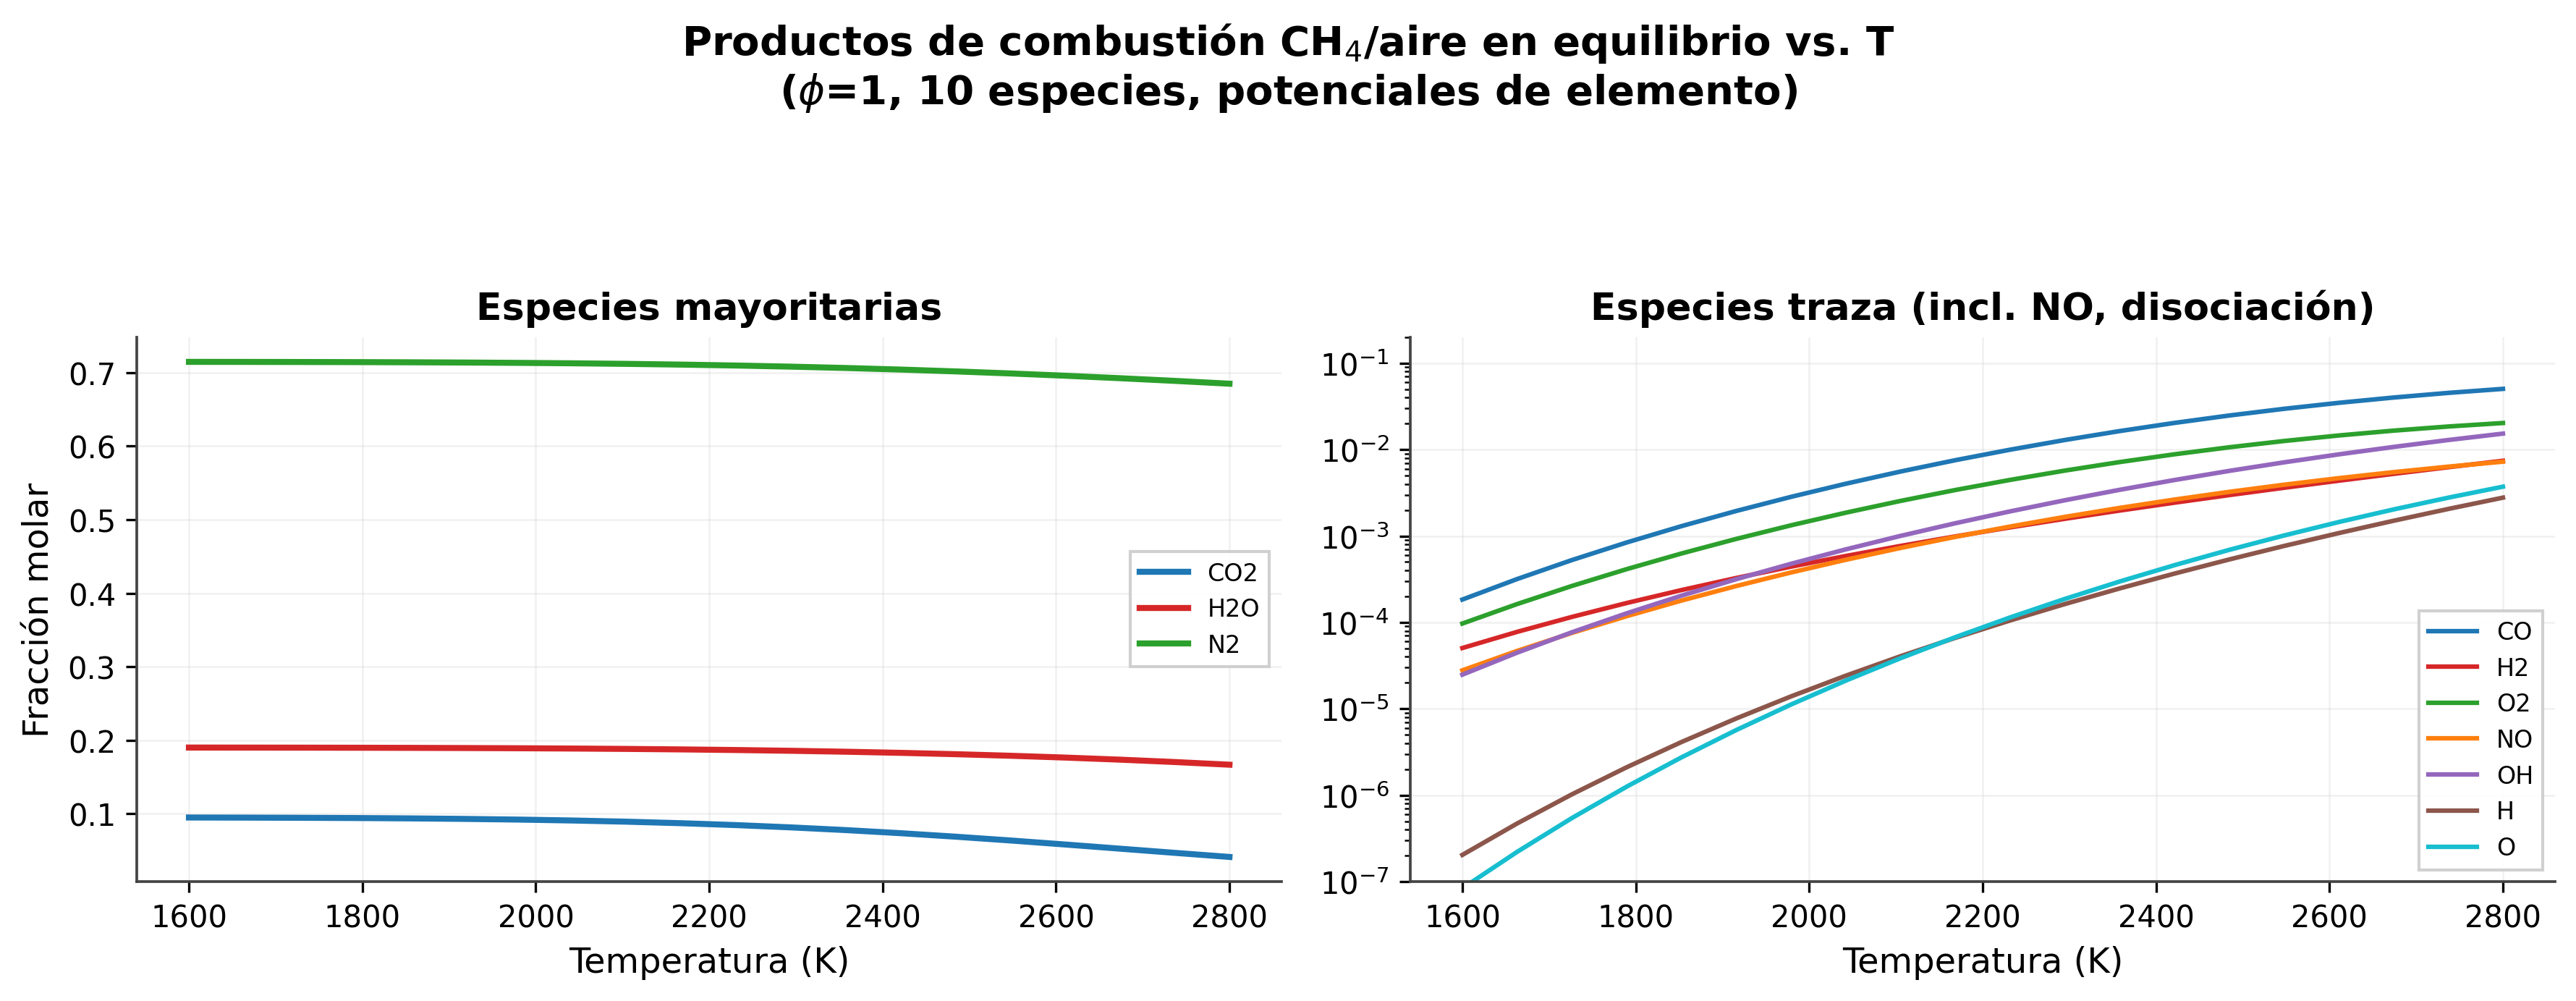
\includegraphics[width=0.95\textwidth]{figuras_exploratorias/E3_llama_CH4_vs_T.png}
\caption{Productos de combustión en equilibrio vs. T, $\phi$=1
(estequiométrico). Izquierda: especies mayoritarias (nótese la ligera
disminución de CO$_2$ y H$_2$O al aumentar T, por disociación hacia
CO/H$_2$/O$_2$). Derecha: especies traza en escala logarítmica,
incluyendo la formación de NO.}
\label{fig:E3}
\end{figure}

\begin{figure}[h]
\centering
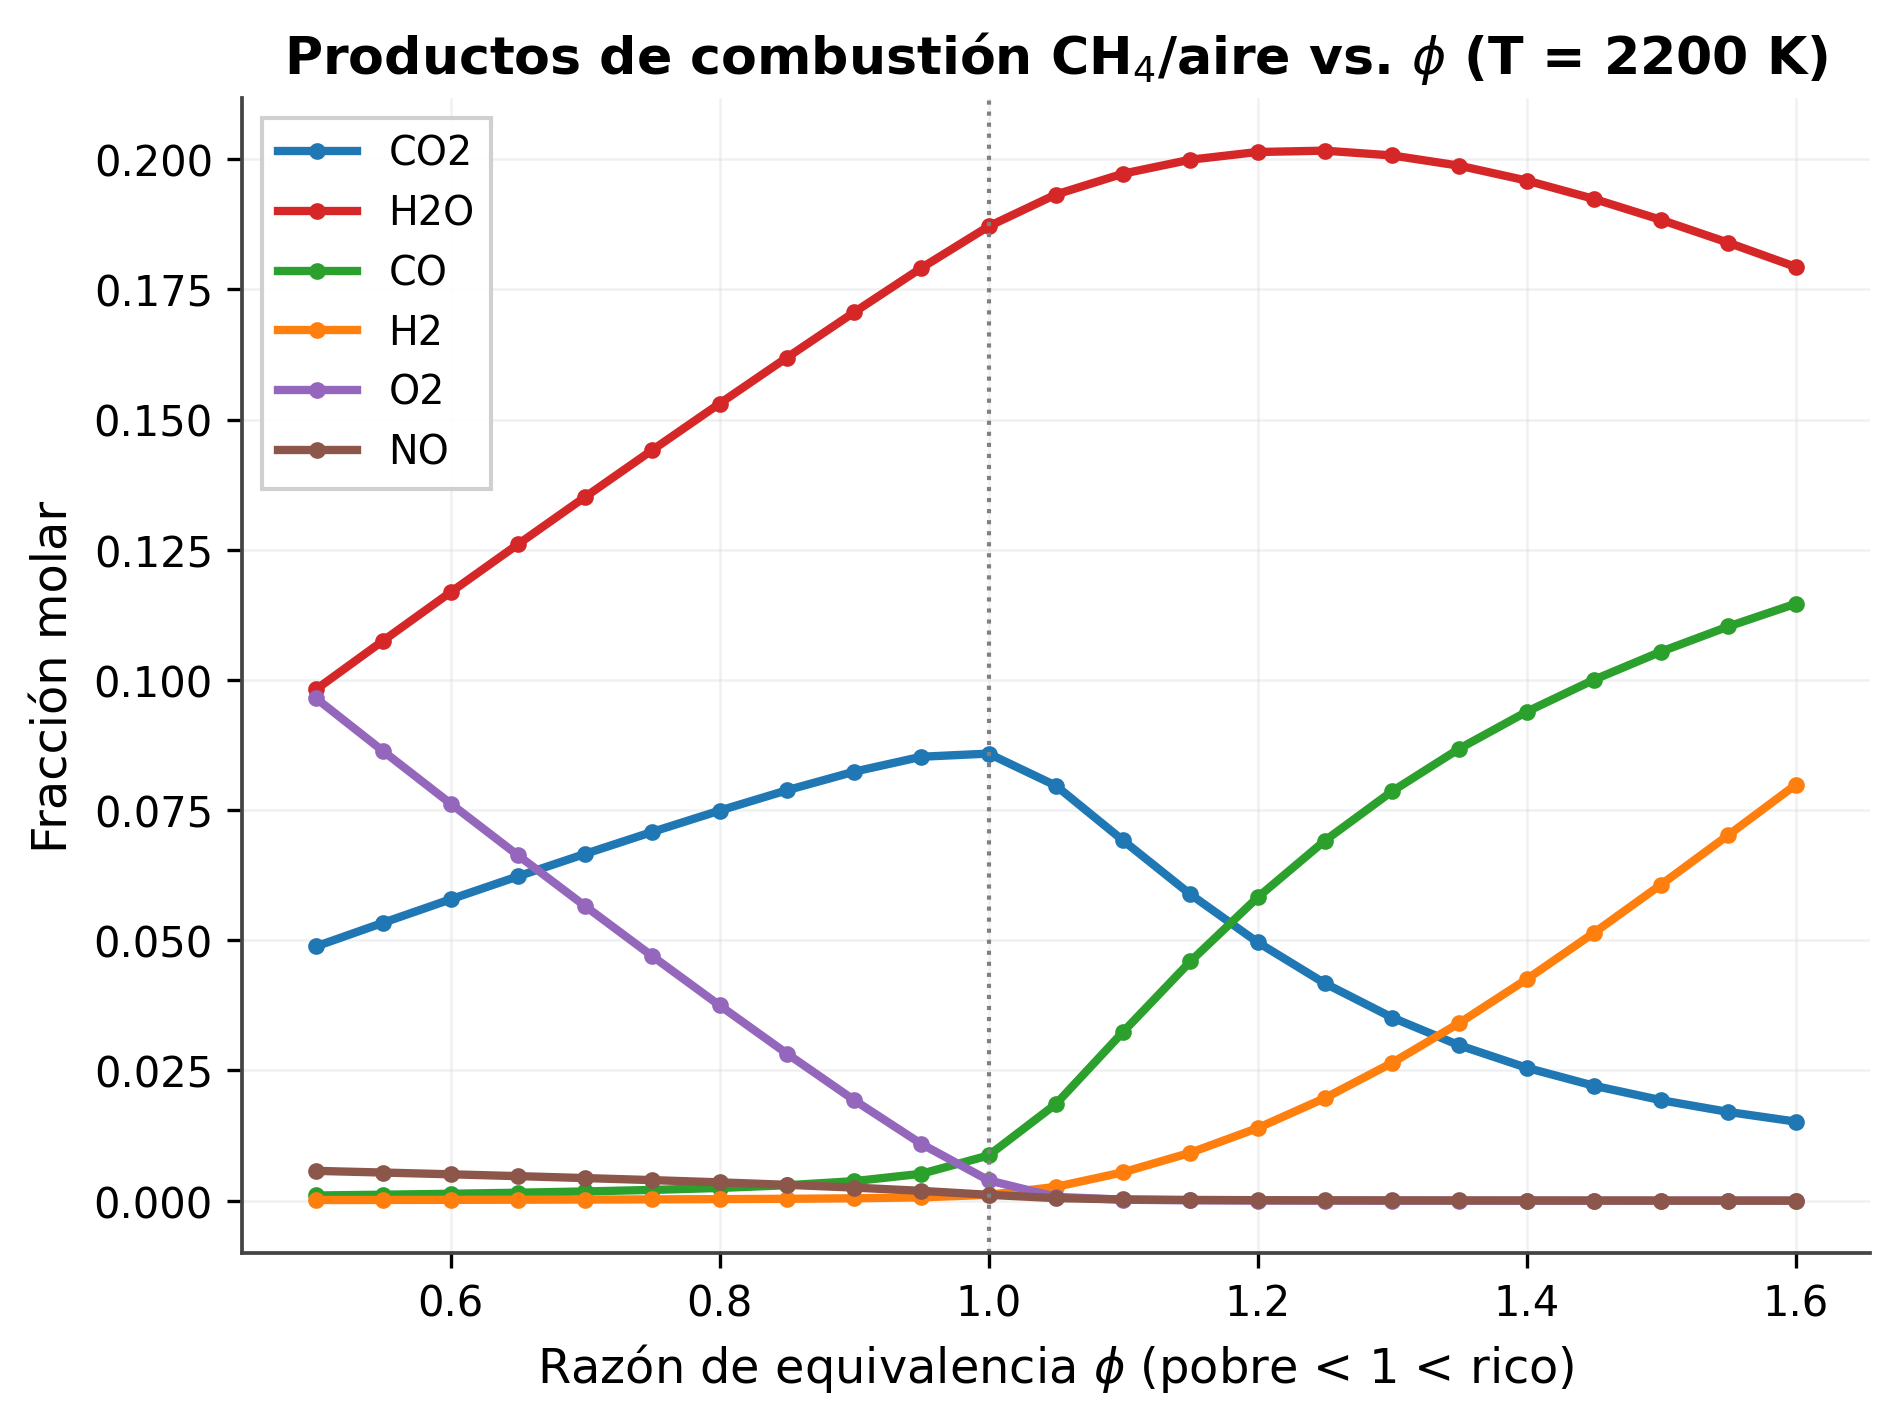
\includegraphics[width=0.68\textwidth]{figuras_exploratorias/E4_llama_CH4_vs_phi.png}
\caption{Productos de combustión vs. razón de equivalencia $\phi$ a
T=2200~K. El comportamiento es cualitativamente idéntico al descrito en
textos de combustión estándar (p. ej. \citet{turns2012}): O$_2$ cae a
cero exactamente en $\phi$=1 hacia adelante, CO y H$_2$ crecen
fuertemente en la zona rica ($\phi>1$, combustión incompleta), y NO se
forma solo donde hay exceso de O$_2$ disponible (zona pobre/cercana a
estequiométrica), consistente con el mecanismo térmico de Zeldovich.}
\label{fig:E4}
\end{figure}

\subsection{Validación cualitativa}

Aunque los valores termoquímicos usados son aproximados, las
\textbf{cuatro} tendencias cualitativas mostradas en
Fig.~\ref{fig:E1}--\ref{fig:E4} coinciden con el comportamiento de
combustión bien establecido en la literatura \citep{turns2012}:
(i)~disociación térmica creciente y abrupta con T; (ii)~orden de
aparición de especies radicales consistente con sus energías de enlace
relativas; (iii)~caída de O$_2$ a cero exactamente en el punto
estequiométrico; (iv)~formación de NO térmico limitada por la
disponibilidad de O$_2$ libre, consistente con el mecanismo de
Zeldovich.

% =====================================================================
\section{Resumen de validaciones}
% =====================================================================

\begin{table}[h]
\centering
\caption{Resumen del nivel de evidencia de cada sección.}
\begin{tabular}{@{}lll@{}}
\toprule
Sección & Sistema & Nivel de evidencia \\
\midrule
\ref{sec:etanol-agua} & VLE etanol-agua & Validado cuantitativamente (azeótropo, $\pm$0.6\%, $\pm$0.2~K) \\
\ref{sec:lle} & LLE solución regular & Demostración matemática (sin referente real) \\
\ref{sec:mtbe} & MTBE reactivo & Consistente internamente (SSA=RAND=scipy, doc. principal) \\
\ref{sec:esterificacion} & Esterificación reactiva & Consistente internamente + $K_{eq}(T)$ validado \\
\ref{sec:combustion} & Combustión CH$_4$/aire, CO$_2$, H$_2$O & Cualitativamente consistente (Le Chatelier, Zeldovich) \\
\bottomrule
\end{tabular}
\end{table}

% =====================================================================
\section{Limitaciones}
% =====================================================================

\begin{itemize}
  \item Los datos termoquímicos de combustión (Sección~\ref{sec:combustion})
    usan $\Delta C_p \approx 0$; una comparación cuantitativa real
    requeriría polinomios NASA-7 o tablas JANAF completas.
  \item El sistema LLE (Sección~\ref{sec:lle}) no corresponde a ningún
    par de compuestos reales.
  \item Los sistemas MTBE y esterificación heredan las mismas
    limitaciones de datos documentadas en \texttt{documentacion.pdf}
    (parámetros de Ung and Doherty y Xiao et al. no disponibles).
  \item El gap de robustez del arranque automático de fases
    (\texttt{documentacion.pdf}, Sección~10.2) sigue sin resolverse;
    todas las figuras de este documento fijan el número de fases de
    antemano para evitarlo.
\end{itemize}

% =====================================================================
\section{Conclusiones}
% =====================================================================

Los solvers validados en \texttt{documentacion.pdf} se aplicaron
exitosamente a cinco sistemas adicionales, produciendo catorce
diagramas termodinámicos. El resultado más destacado es que, sin
ningún ajuste, el modelo UNIFAC predice el azeótropo etanol-agua con
precisión notable. Los perfiles de combustión, aunque basados en datos
termoquímicos aproximados, reproducen correctamente las tendencias
cualitativas centrales de la química de combustión a alta temperatura.
En conjunto, estos resultados sugieren que la implementación no solo es
matemáticamente correcta (ver \texttt{documentacion.pdf}) sino que
produce predicciones físicamente razonables al aplicarse a sistemas
diversos.

% =====================================================================
\bibliographystyle{plainnat}
\bibliography{referencias}

\end{document}
